\documentclass[12pt, a4paper, oneside]{article}
\usepackage{amsmath, amsthm, amssymb, appendix, bm, graphicx, hyperref, mathrsfs, makecell}
\usepackage{bbm, stfloats, subfigure, pythonhighlight, CJK, algorithm, algorithmicx, algpseudocode}
\usepackage{geometry}
\geometry{a4paper,left=2.5cm,right=2.5cm,top=3cm,bottom=3cm}
\usepackage{fancyhdr}
\pagestyle{fancy}
\renewcommand\headrulewidth{.5pt}
\renewcommand\footrulewidth{0pt}
\setlength{\headheight}{15pt}
\fancyhead[L]{\textit{\leftmark}}
\fancyhead[R]{\thepage}

\title{\textbf{Federated CP New Setting}}
\author{Min}
\date{\today}
\linespread{1.6}
\definecolor{lightBlue}{rgb}{0.274,0.41,0.879}
\definecolor{darckGreen}{rgb}{0.1797,0.543,0.3398}
%{\color{lightBlue}Text Here}
\newtheorem{theorem}{Theorem}[section]
\newtheorem{definition}[theorem]{Definition}
\newtheorem{lemma}[theorem]{Lemma}
\newtheorem{corollary}[theorem]{Corollary}
\newtheorem{example}[theorem]{Example}
\newtheorem{proposition}[theorem]{Proposition}
\newtheorem{remark}[theorem]{Remark}
\renewcommand{\abstractname}{\Large\textbf{Abstract}}
\floatname{algorithm}{Algorithm}
\renewcommand{\algorithmicrequire}{\textbf{Input:}}
\renewcommand{\algorithmicensure}{\textbf{Output:}}

\begin{document}
\maketitle
\tableofcontents
\setcounter{page}{1}
\pagenumbering{arabic}
\section{Idea1}
    For $K$ agents each with $Z_k=\{(X_i^k,Y_i^k)\}_{i=1}^{n_k}$ sampled from distribution $P^k$, and point predictor $f_1$ based score $S_i^k$. If all $P^k=P$ and a new test point $X,Y$ from $P^1$. For any trial data $y$ and score $S$ follow the procedure in "Conformal prediction with local weights: randomization enables robust guarantees"\cite{hore2023conformal}:
    \begin{itemize}
        \item Find some kernel function $H(\cdot,\cdot)$, sample $\tilde{X}$ based on $H(X,\cdot)$.
        \item Calculate empirical function $\tilde{F}=\overset{}{\underset{i,k}\sum}w_i^k\delta_{S_i^k}+w\delta_{S}$ with weight
        \begin{equation*}
            w_i^k=\dfrac{H(X_i^k,\tilde{X})}{\overset{}{\underset{i',k'}\sum}H(X_{i'}^{k'},\tilde{X})+H(X,\tilde{X})},\ w=\dfrac{H(X,\tilde{X})}{\overset{}{\underset{i',k'}\sum}H(X_{i'}^{k'},\tilde{X})+H(X,\tilde{X})}.
        \end{equation*}
        \item Conformal set is $C_\alpha(X)=\{S\leq Q(1-\alpha,\tilde{F})\}$.
    \end{itemize}


    However for all $k$ $P^k=P$ is not practical, potential covariate shift exists

\subsection{Experiment1}
    Assume agent $k=1,\cdots,K$ each has $n$ samples $X_1^k,\cdots,X_n^k$ follow $N(\mu_k,9)$. Sythesize $Y_i^k=(X_i^k)^2+\epsilon$, where $\epsilon\sim N(0,(ep*|X|)^2)$, $ep$ be some parameter. Under this problem only have covariate shift.

    \begin{itemize}
        \item $X$ has different distribution for each agents
        \item $EY|X$ is same for all agents
        \item $Y-EY|X$ has same distribution for all agents
    \end{itemize}
    

    Covariate shift has little influence on this method as the method is localized. More on Fig \ref{Fig1}. $ep=h=0.5$
    \begin{figure}[htbp]
        \centering
        \begin{minipage}{0.495\linewidth}
            \centering
            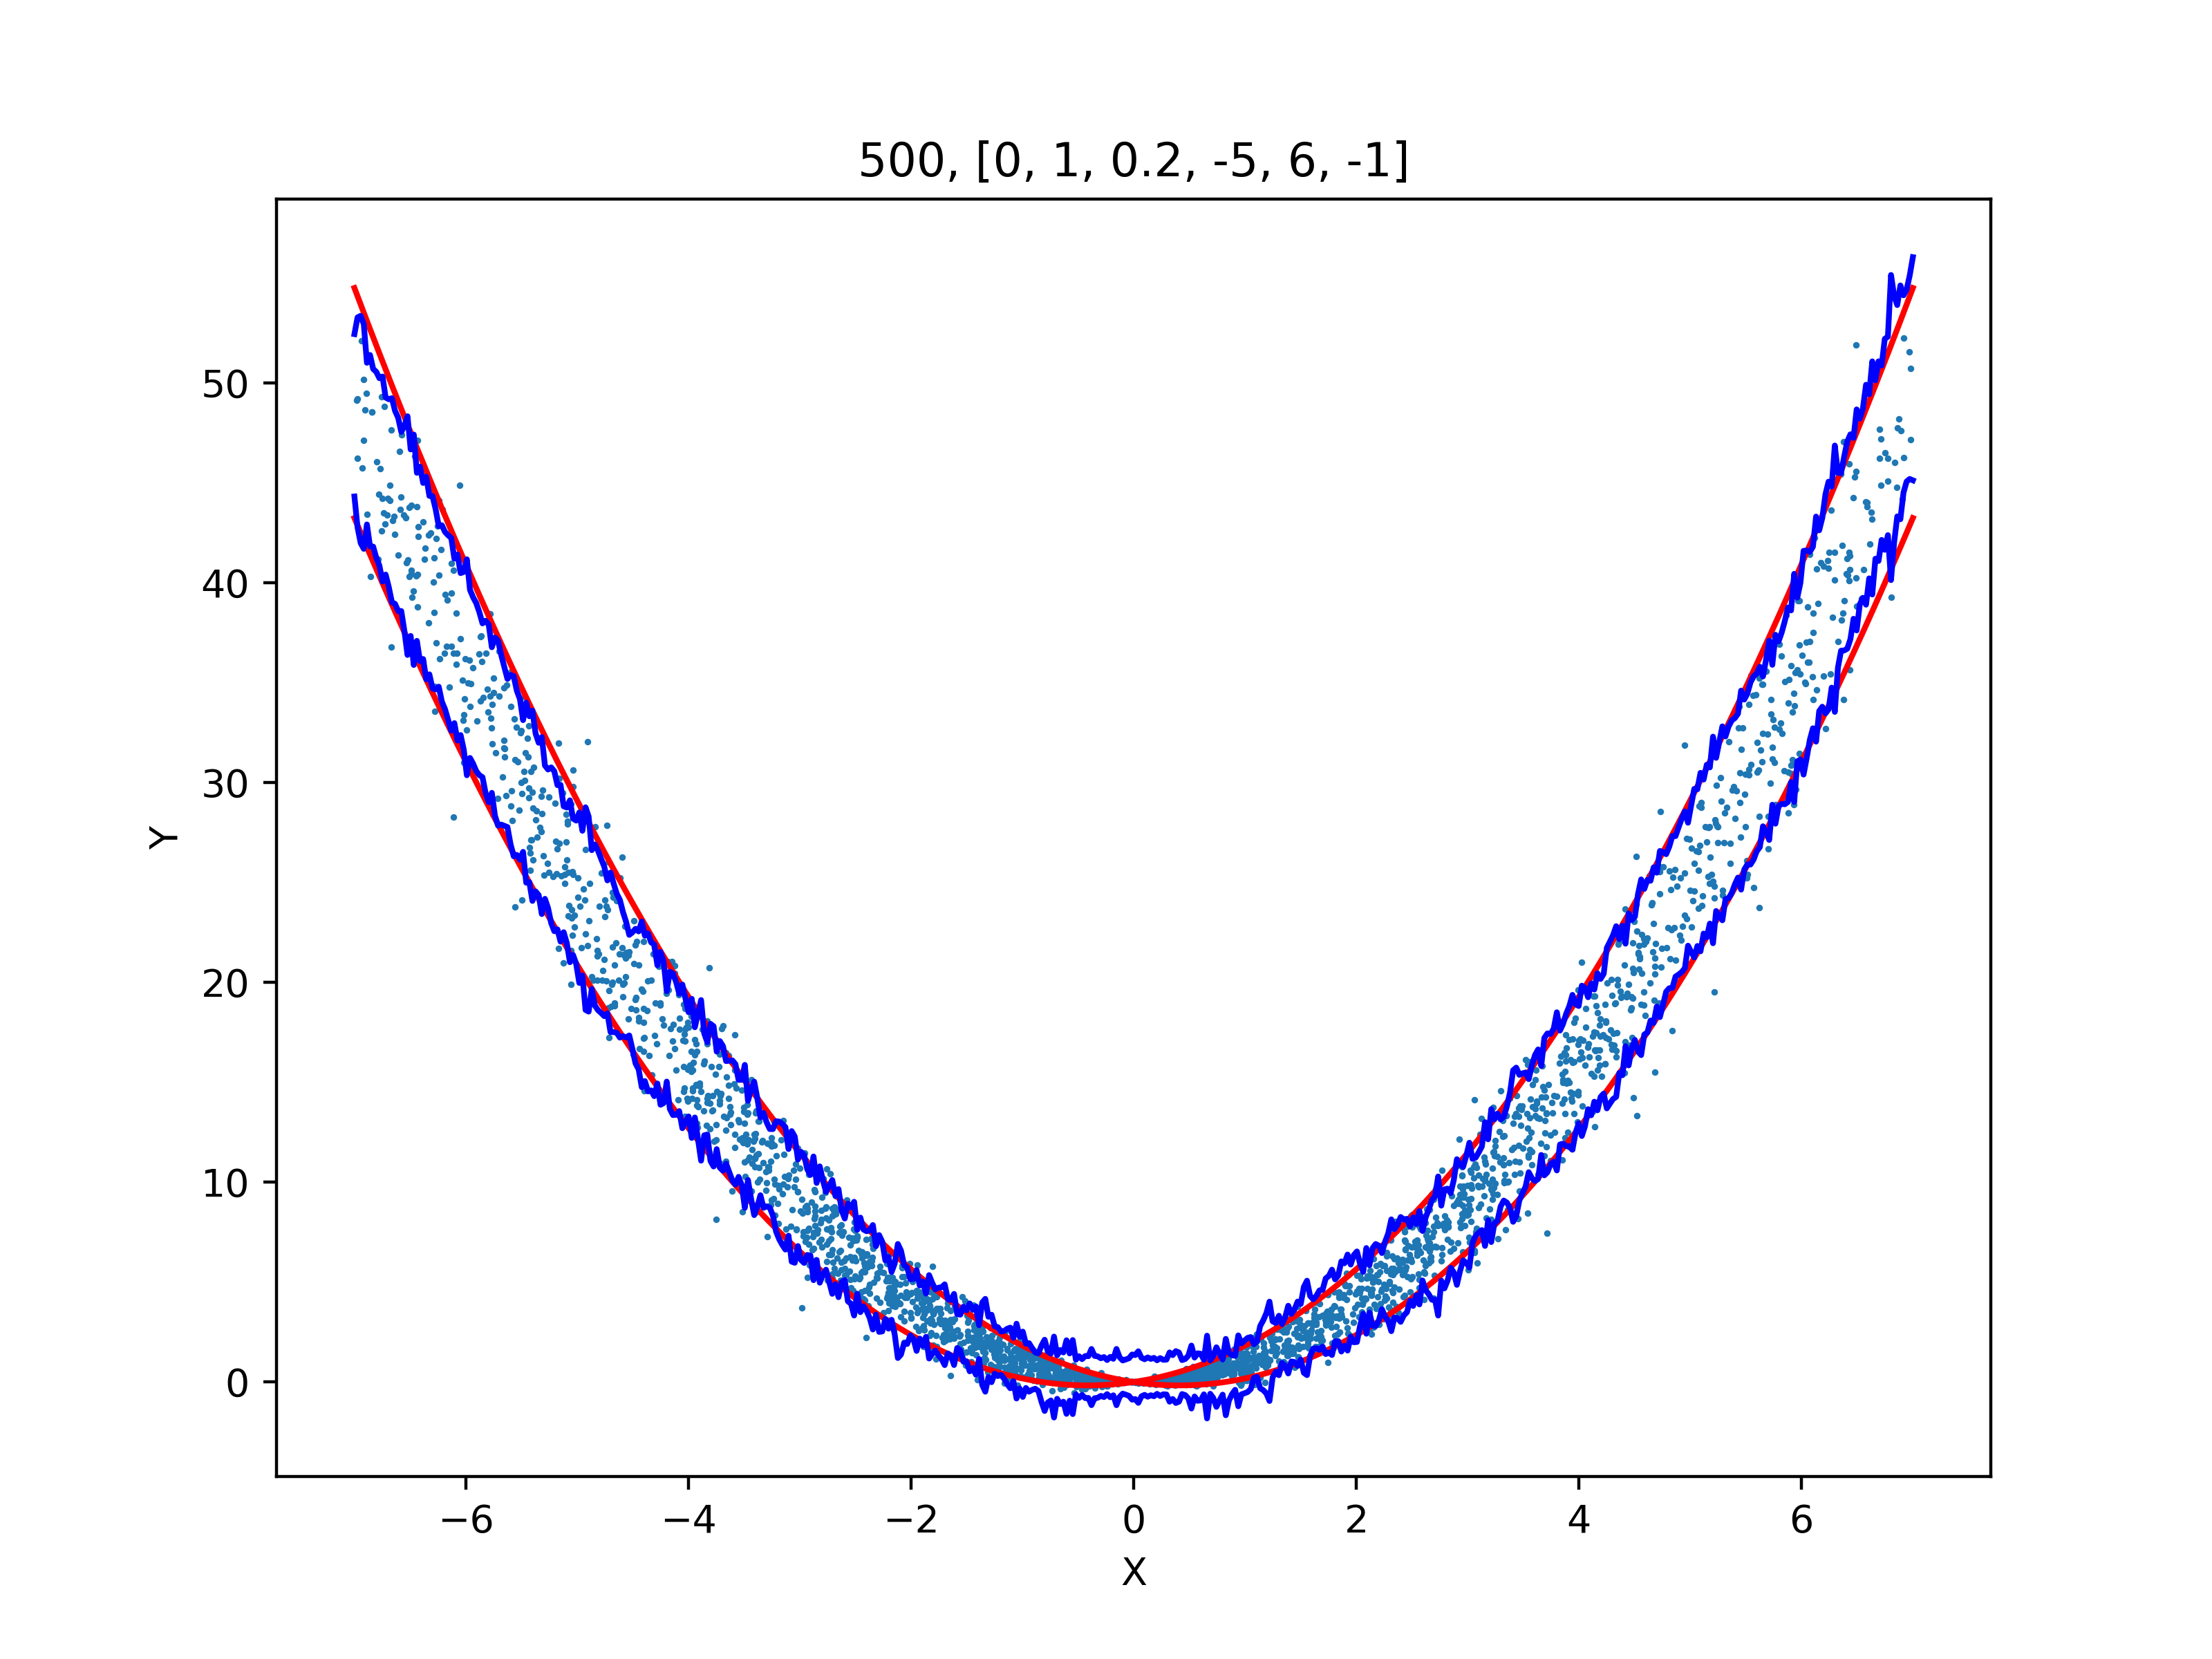
\includegraphics[width=0.98\linewidth]{fig/Ex1_1/0_1_.png}
        \end{minipage}
        \begin{minipage}{0.495\linewidth}
            \centering
            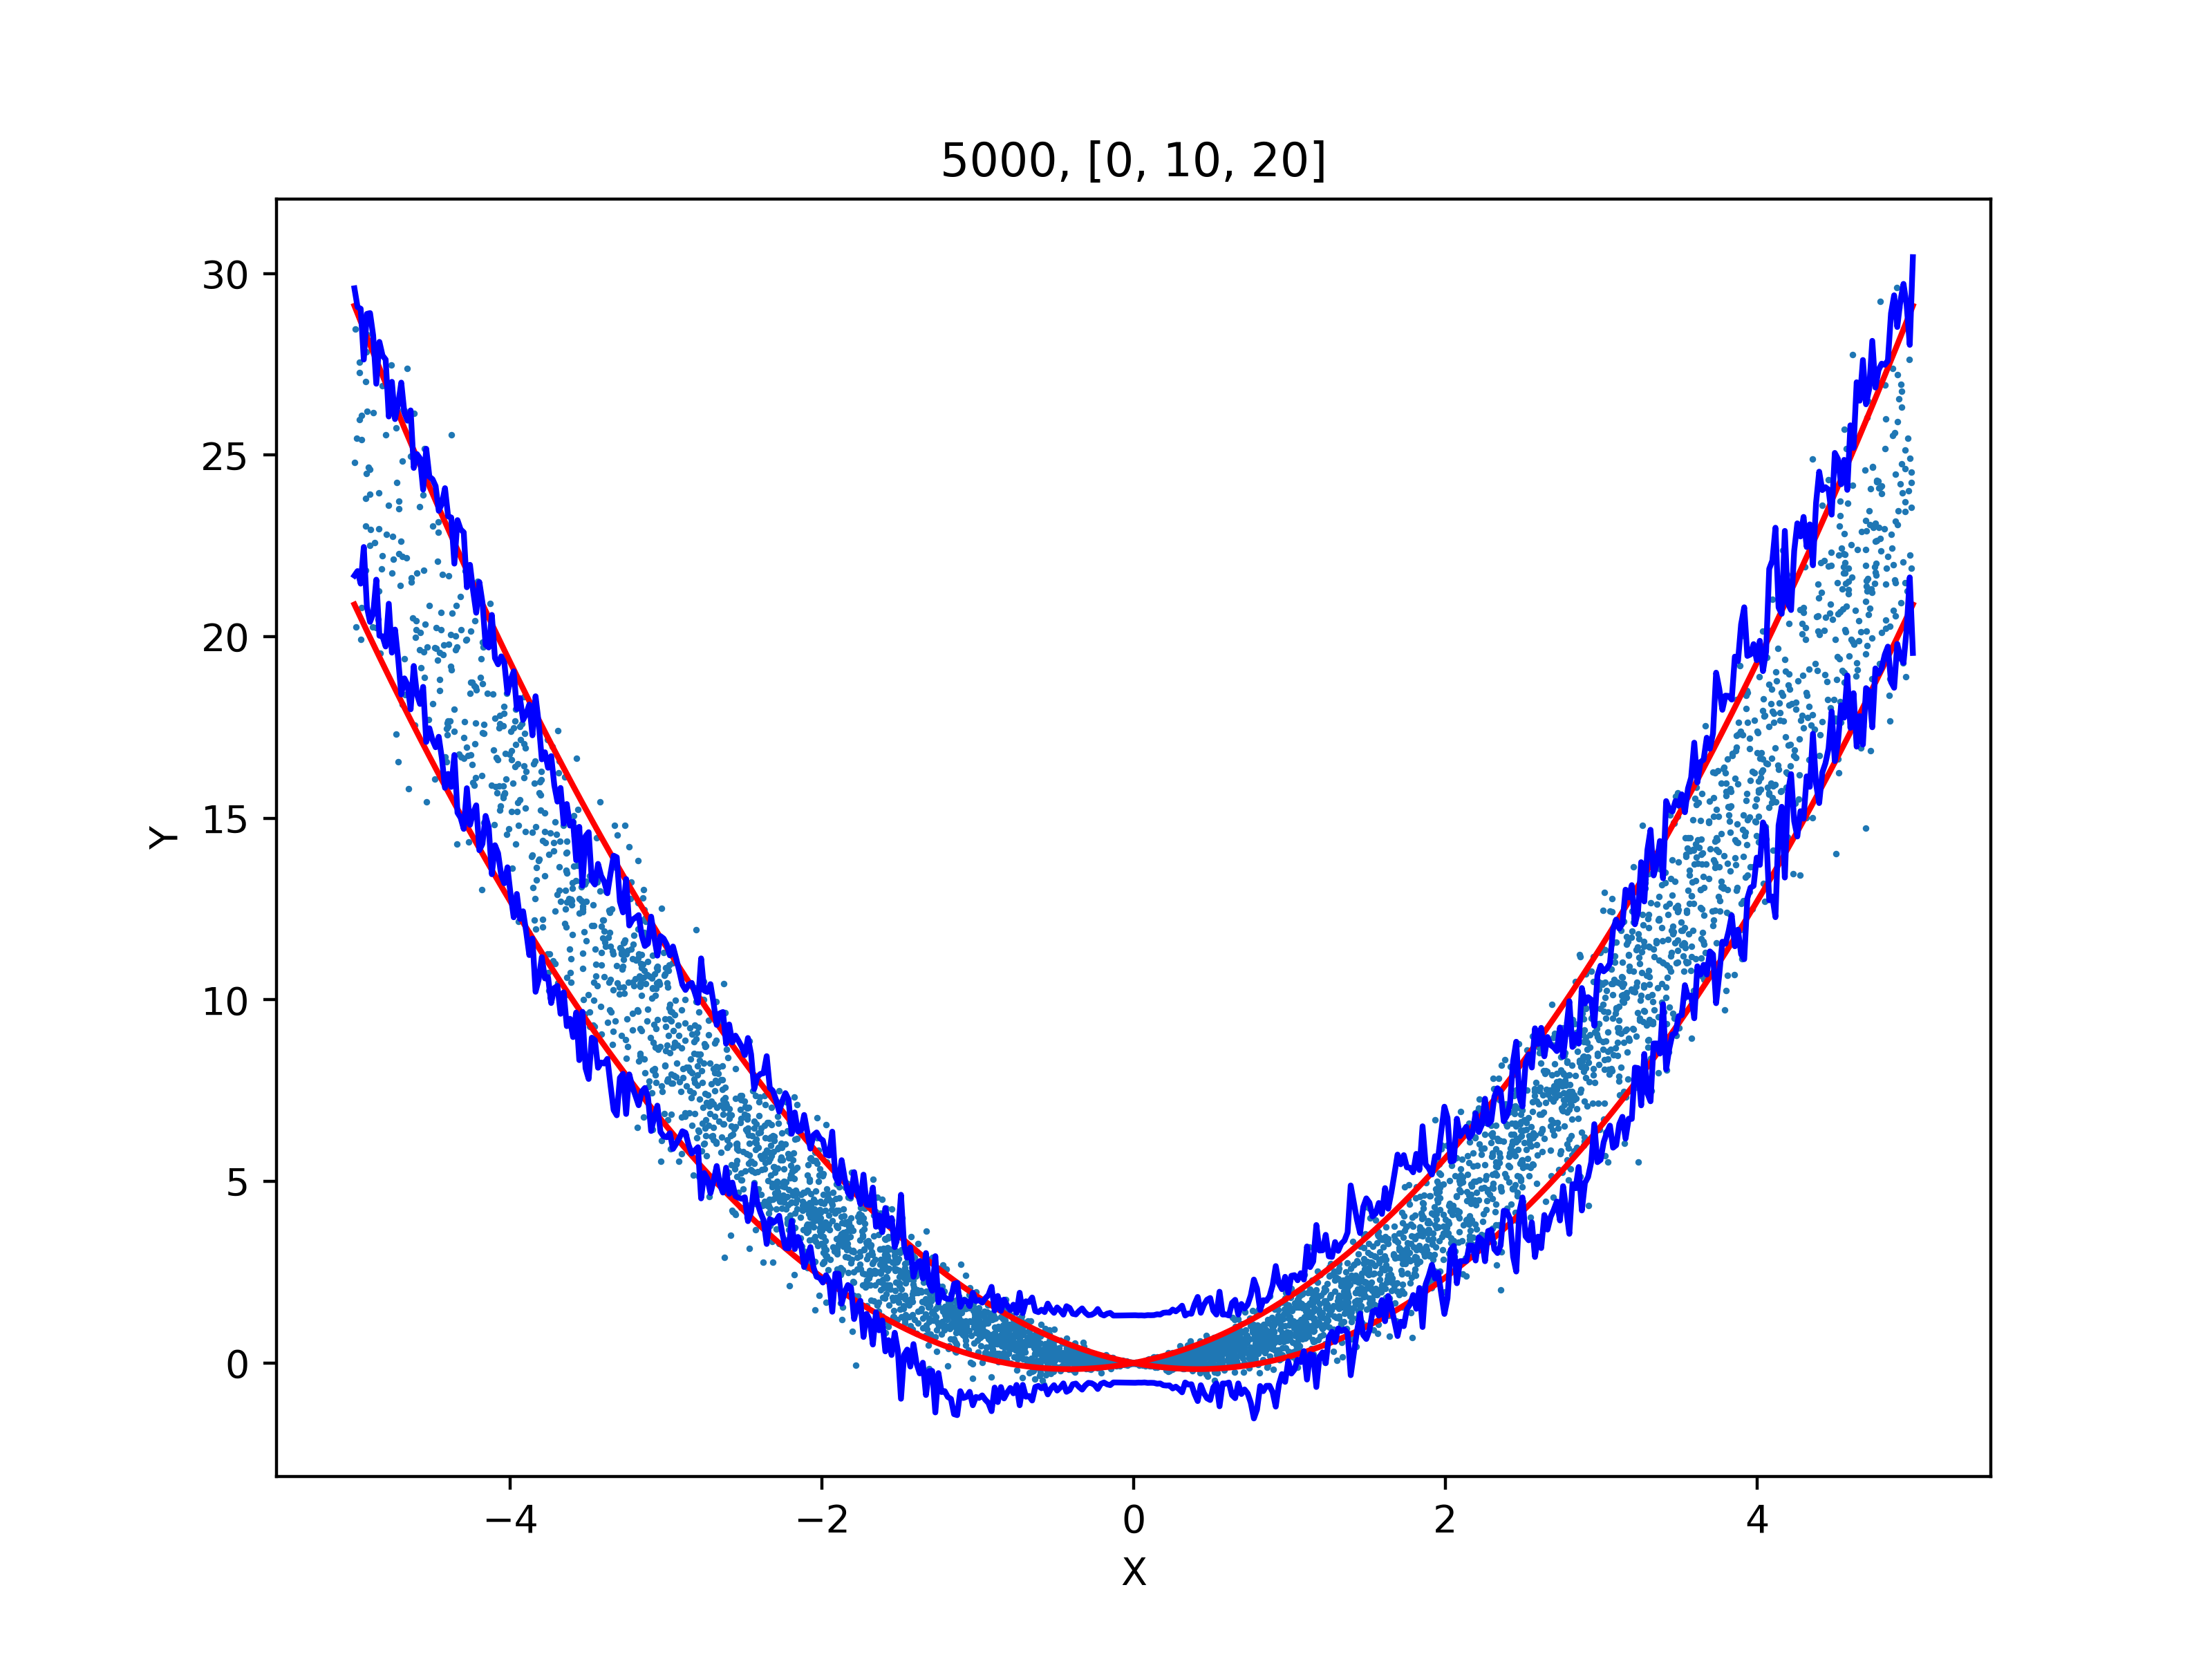
\includegraphics[width=0.98\linewidth]{fig/Ex1_1/0_10_20.png}
        \end{minipage}
        \centering
        \begin{minipage}{0.495\linewidth}
            \centering
            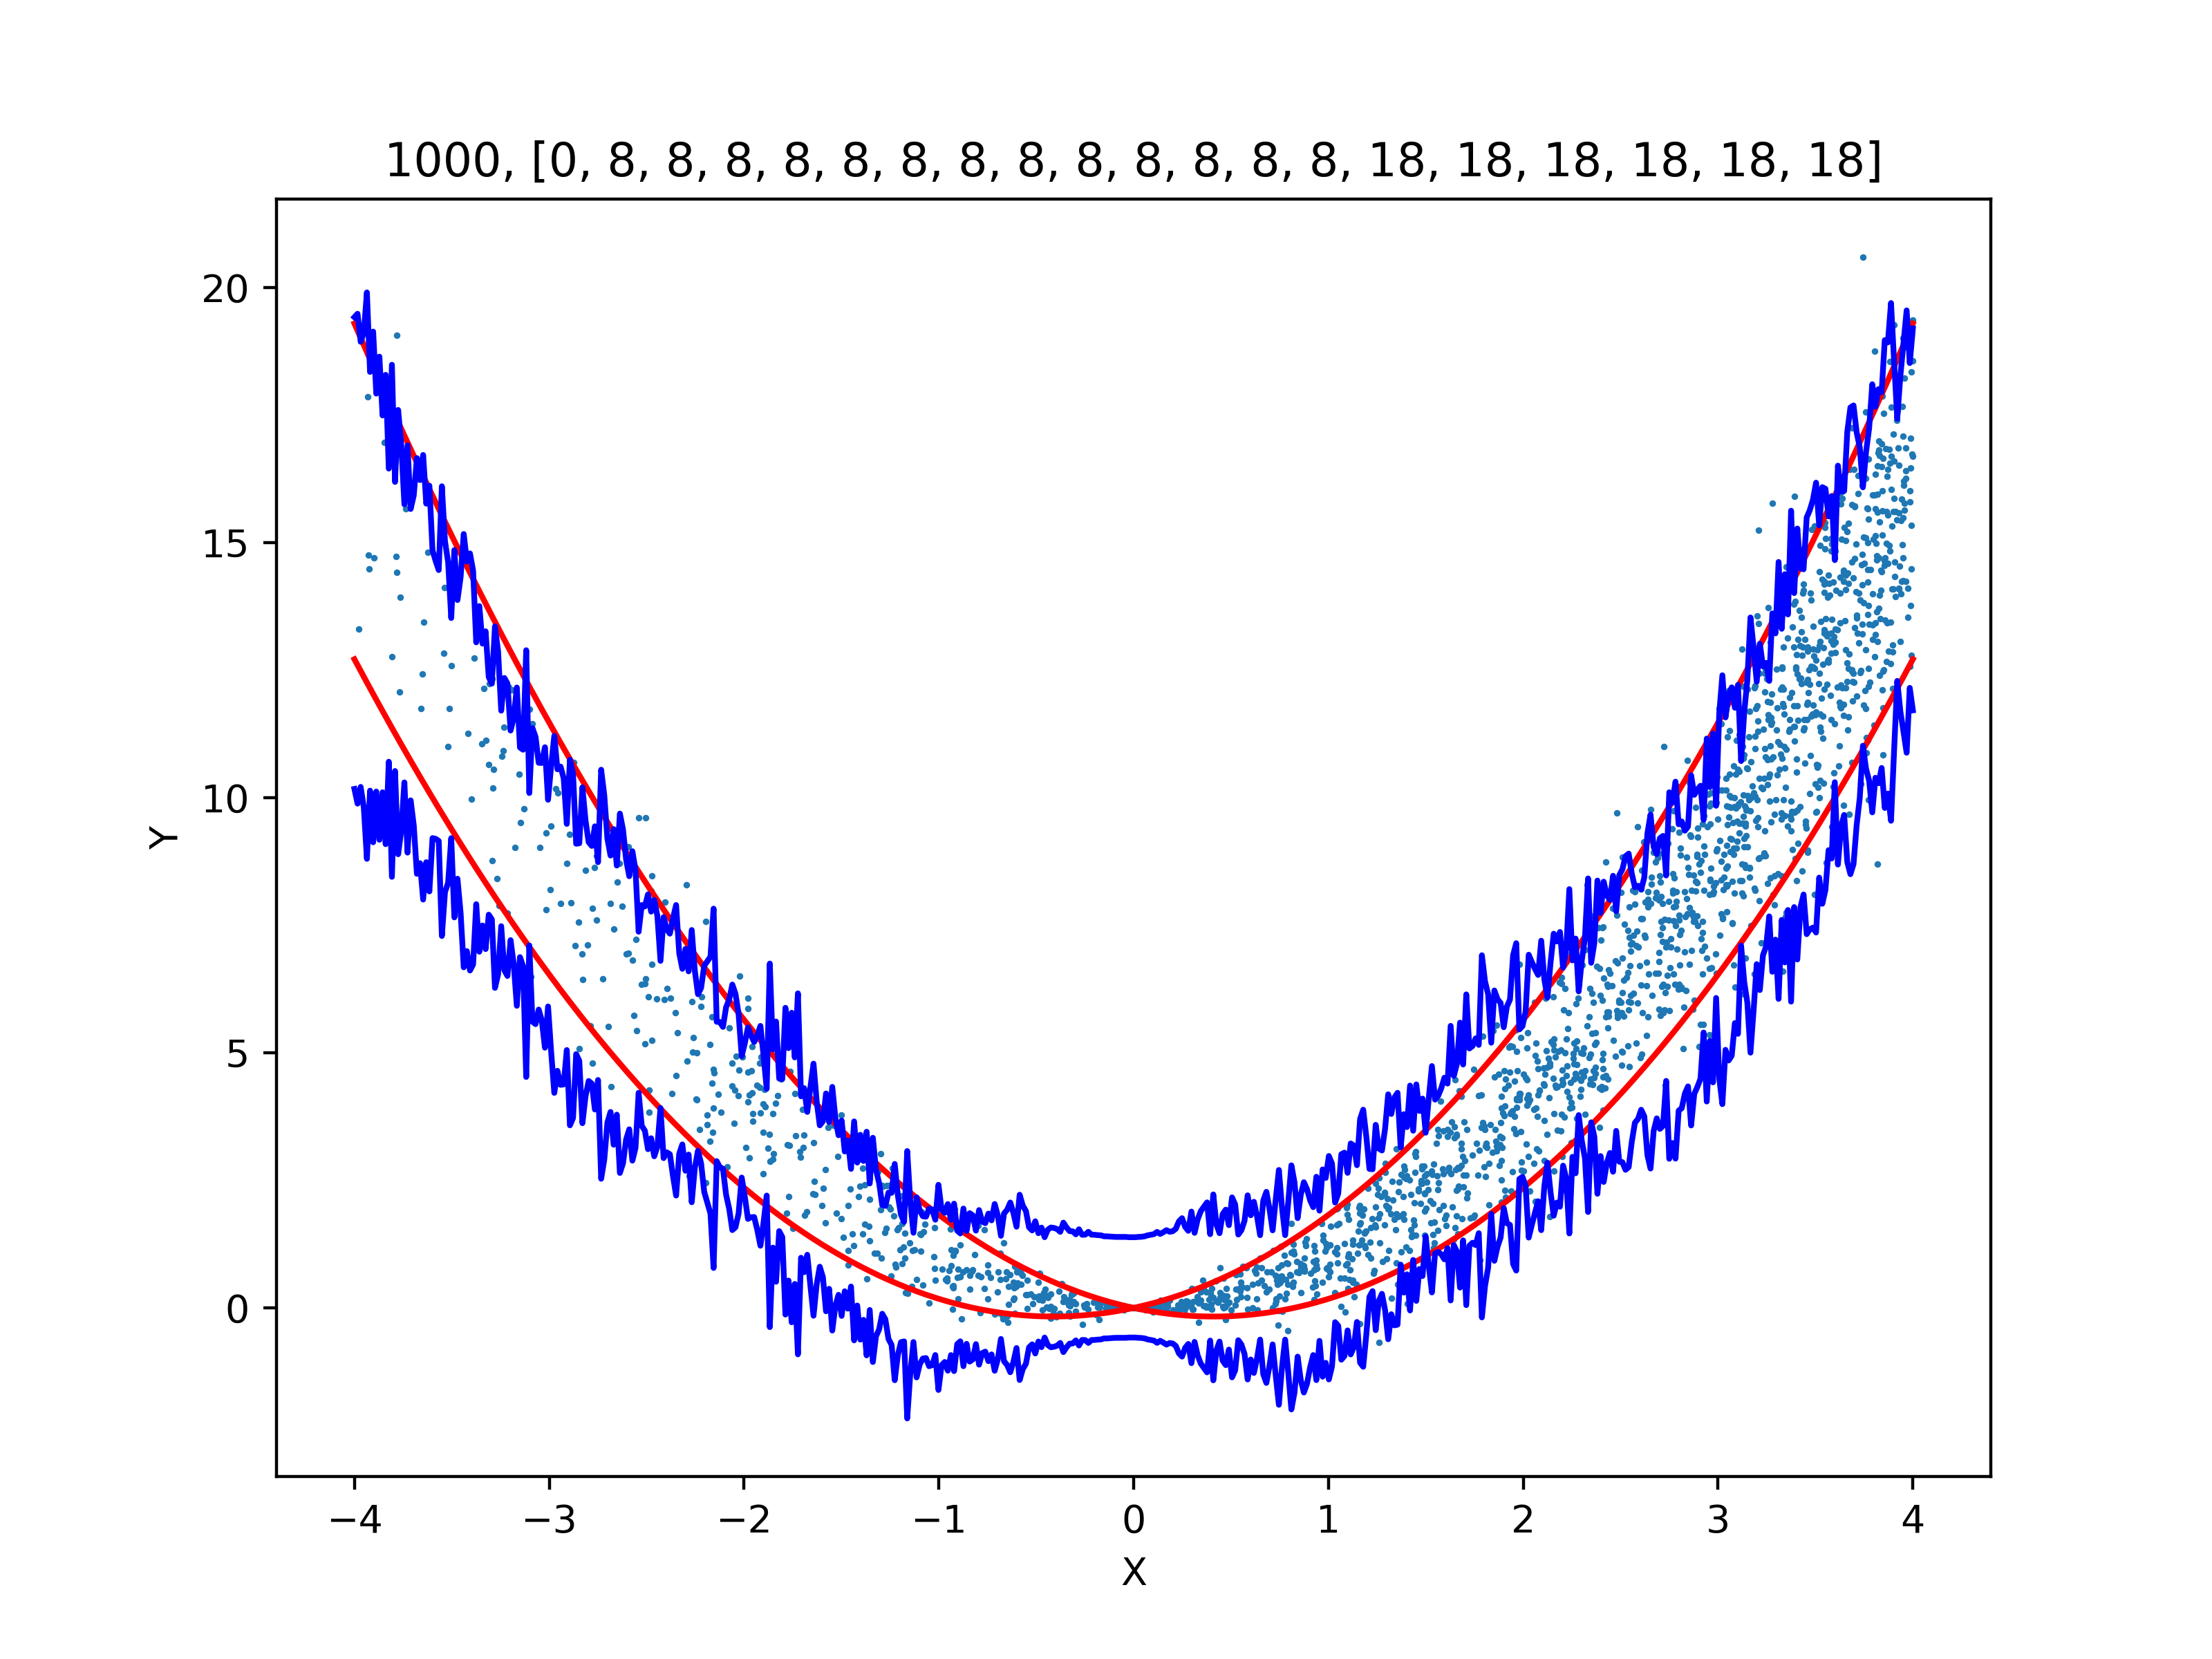
\includegraphics[width=0.98\linewidth]{fig/Ex1_1/0_8_18.png}
        \end{minipage}
        \begin{minipage}{0.495\linewidth}
            \centering
            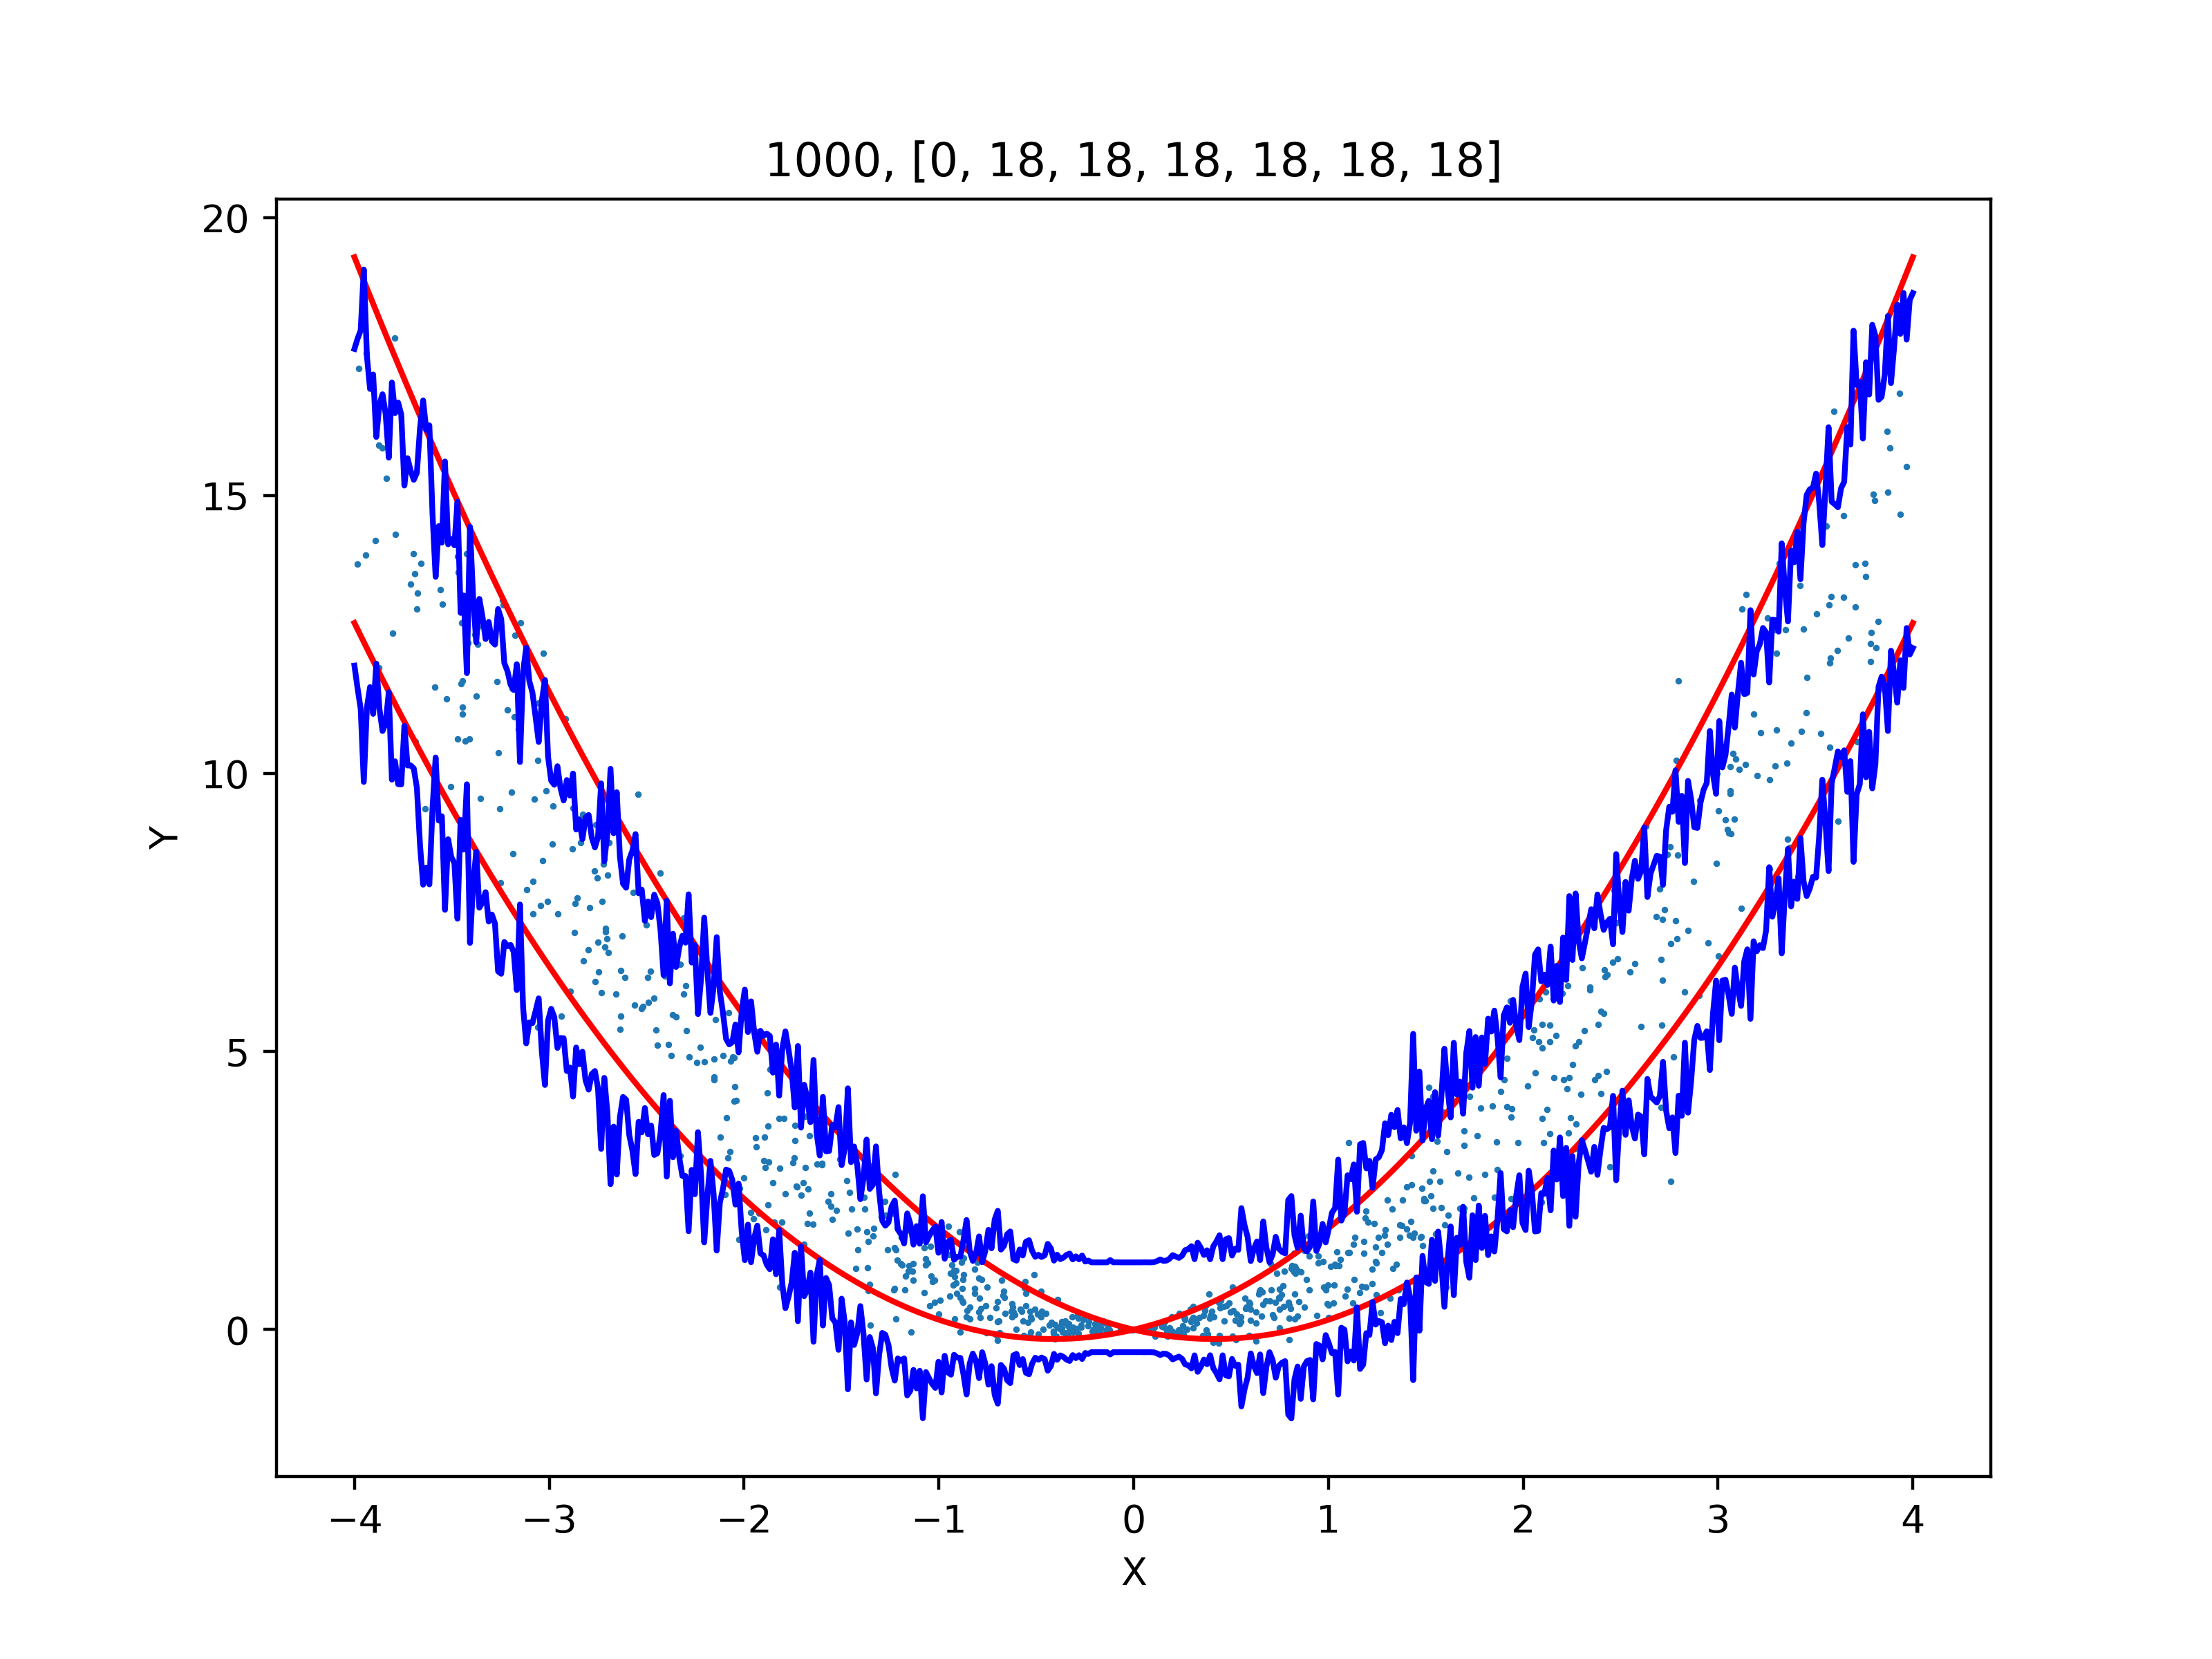
\includegraphics[width=0.98\linewidth]{fig/Ex1_1/0_18.png}
        \end{minipage}
        \caption{Fig1}
        \label{Fig1}
    \end{figure}

    Generate 1000 samples with location 0, and 1000 samples with location 0 and 20. The left shows the performance on only within samples with 0 location and 1000 samples is better than the right one using 2000 data samples. This comes from covariate shift, the scores from samples with location 20 influences origin behavior, from Fig \ref{Fig2}
    \begin{figure}[htbp]
        \centering
        \begin{minipage}{0.495\linewidth}
            \centering
            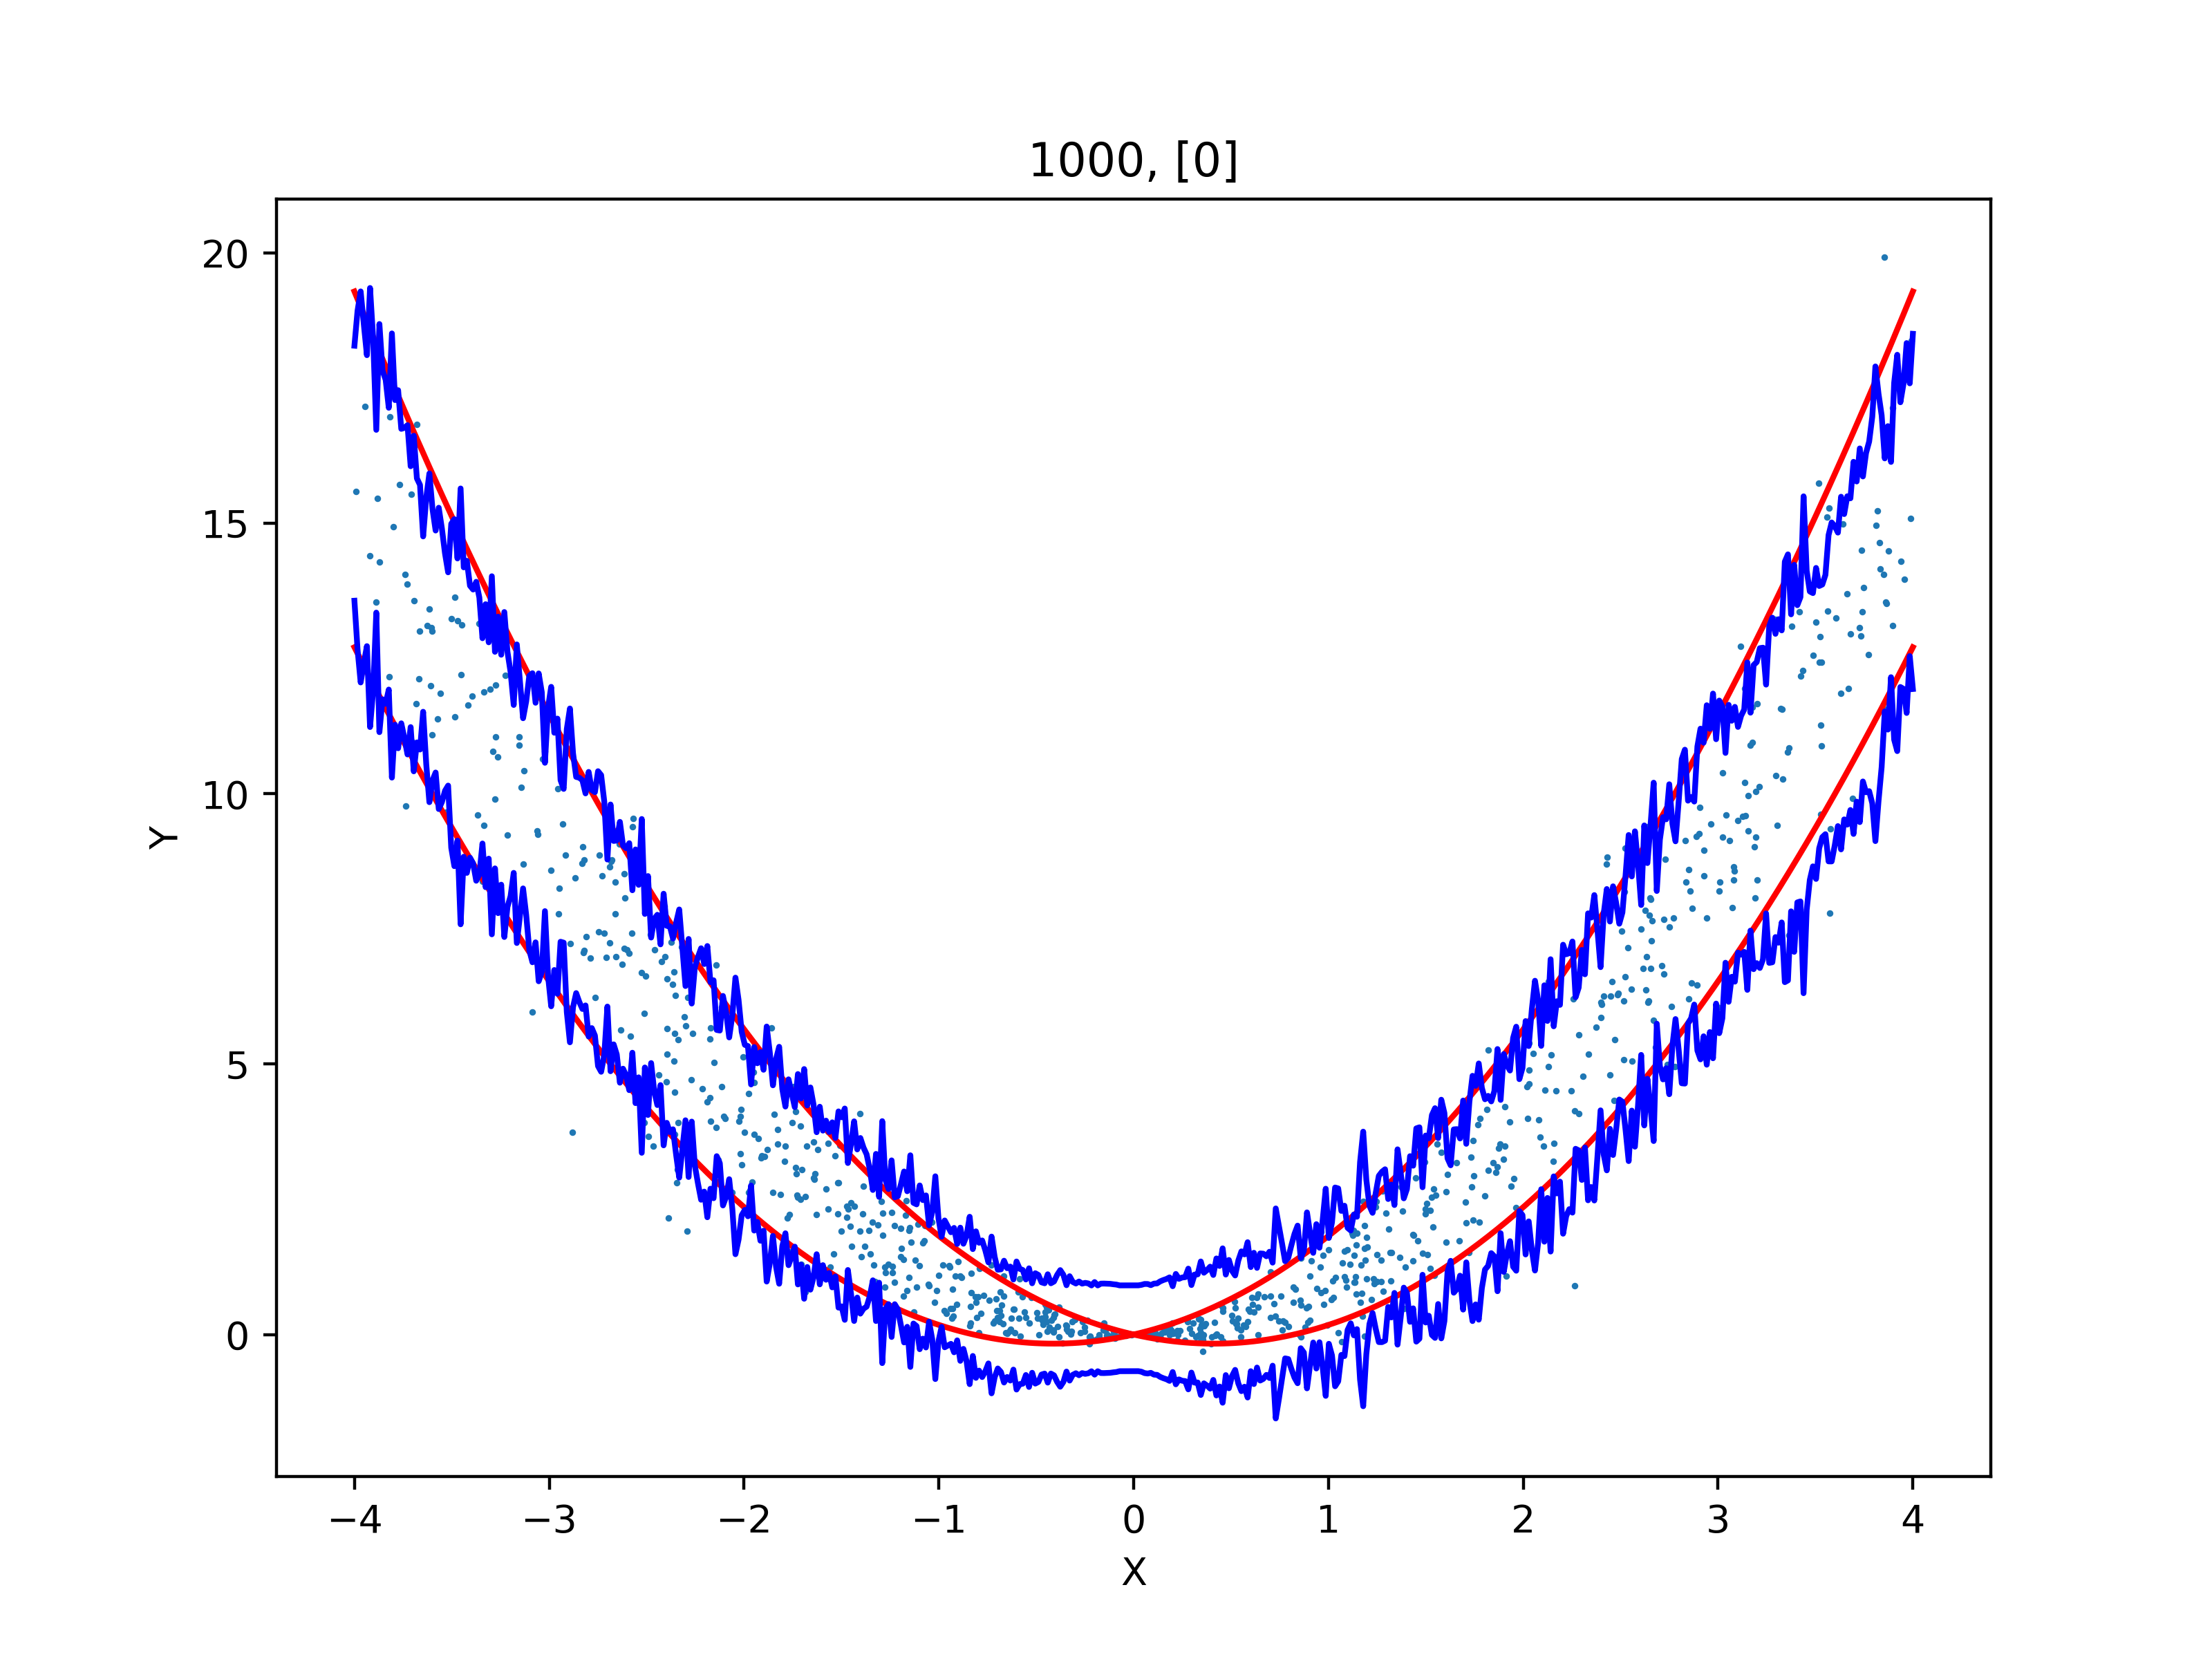
\includegraphics[width=0.98\linewidth]{fig/Ex1_1/0.png}
        \end{minipage}
        \begin{minipage}{0.495\linewidth}
            \centering
            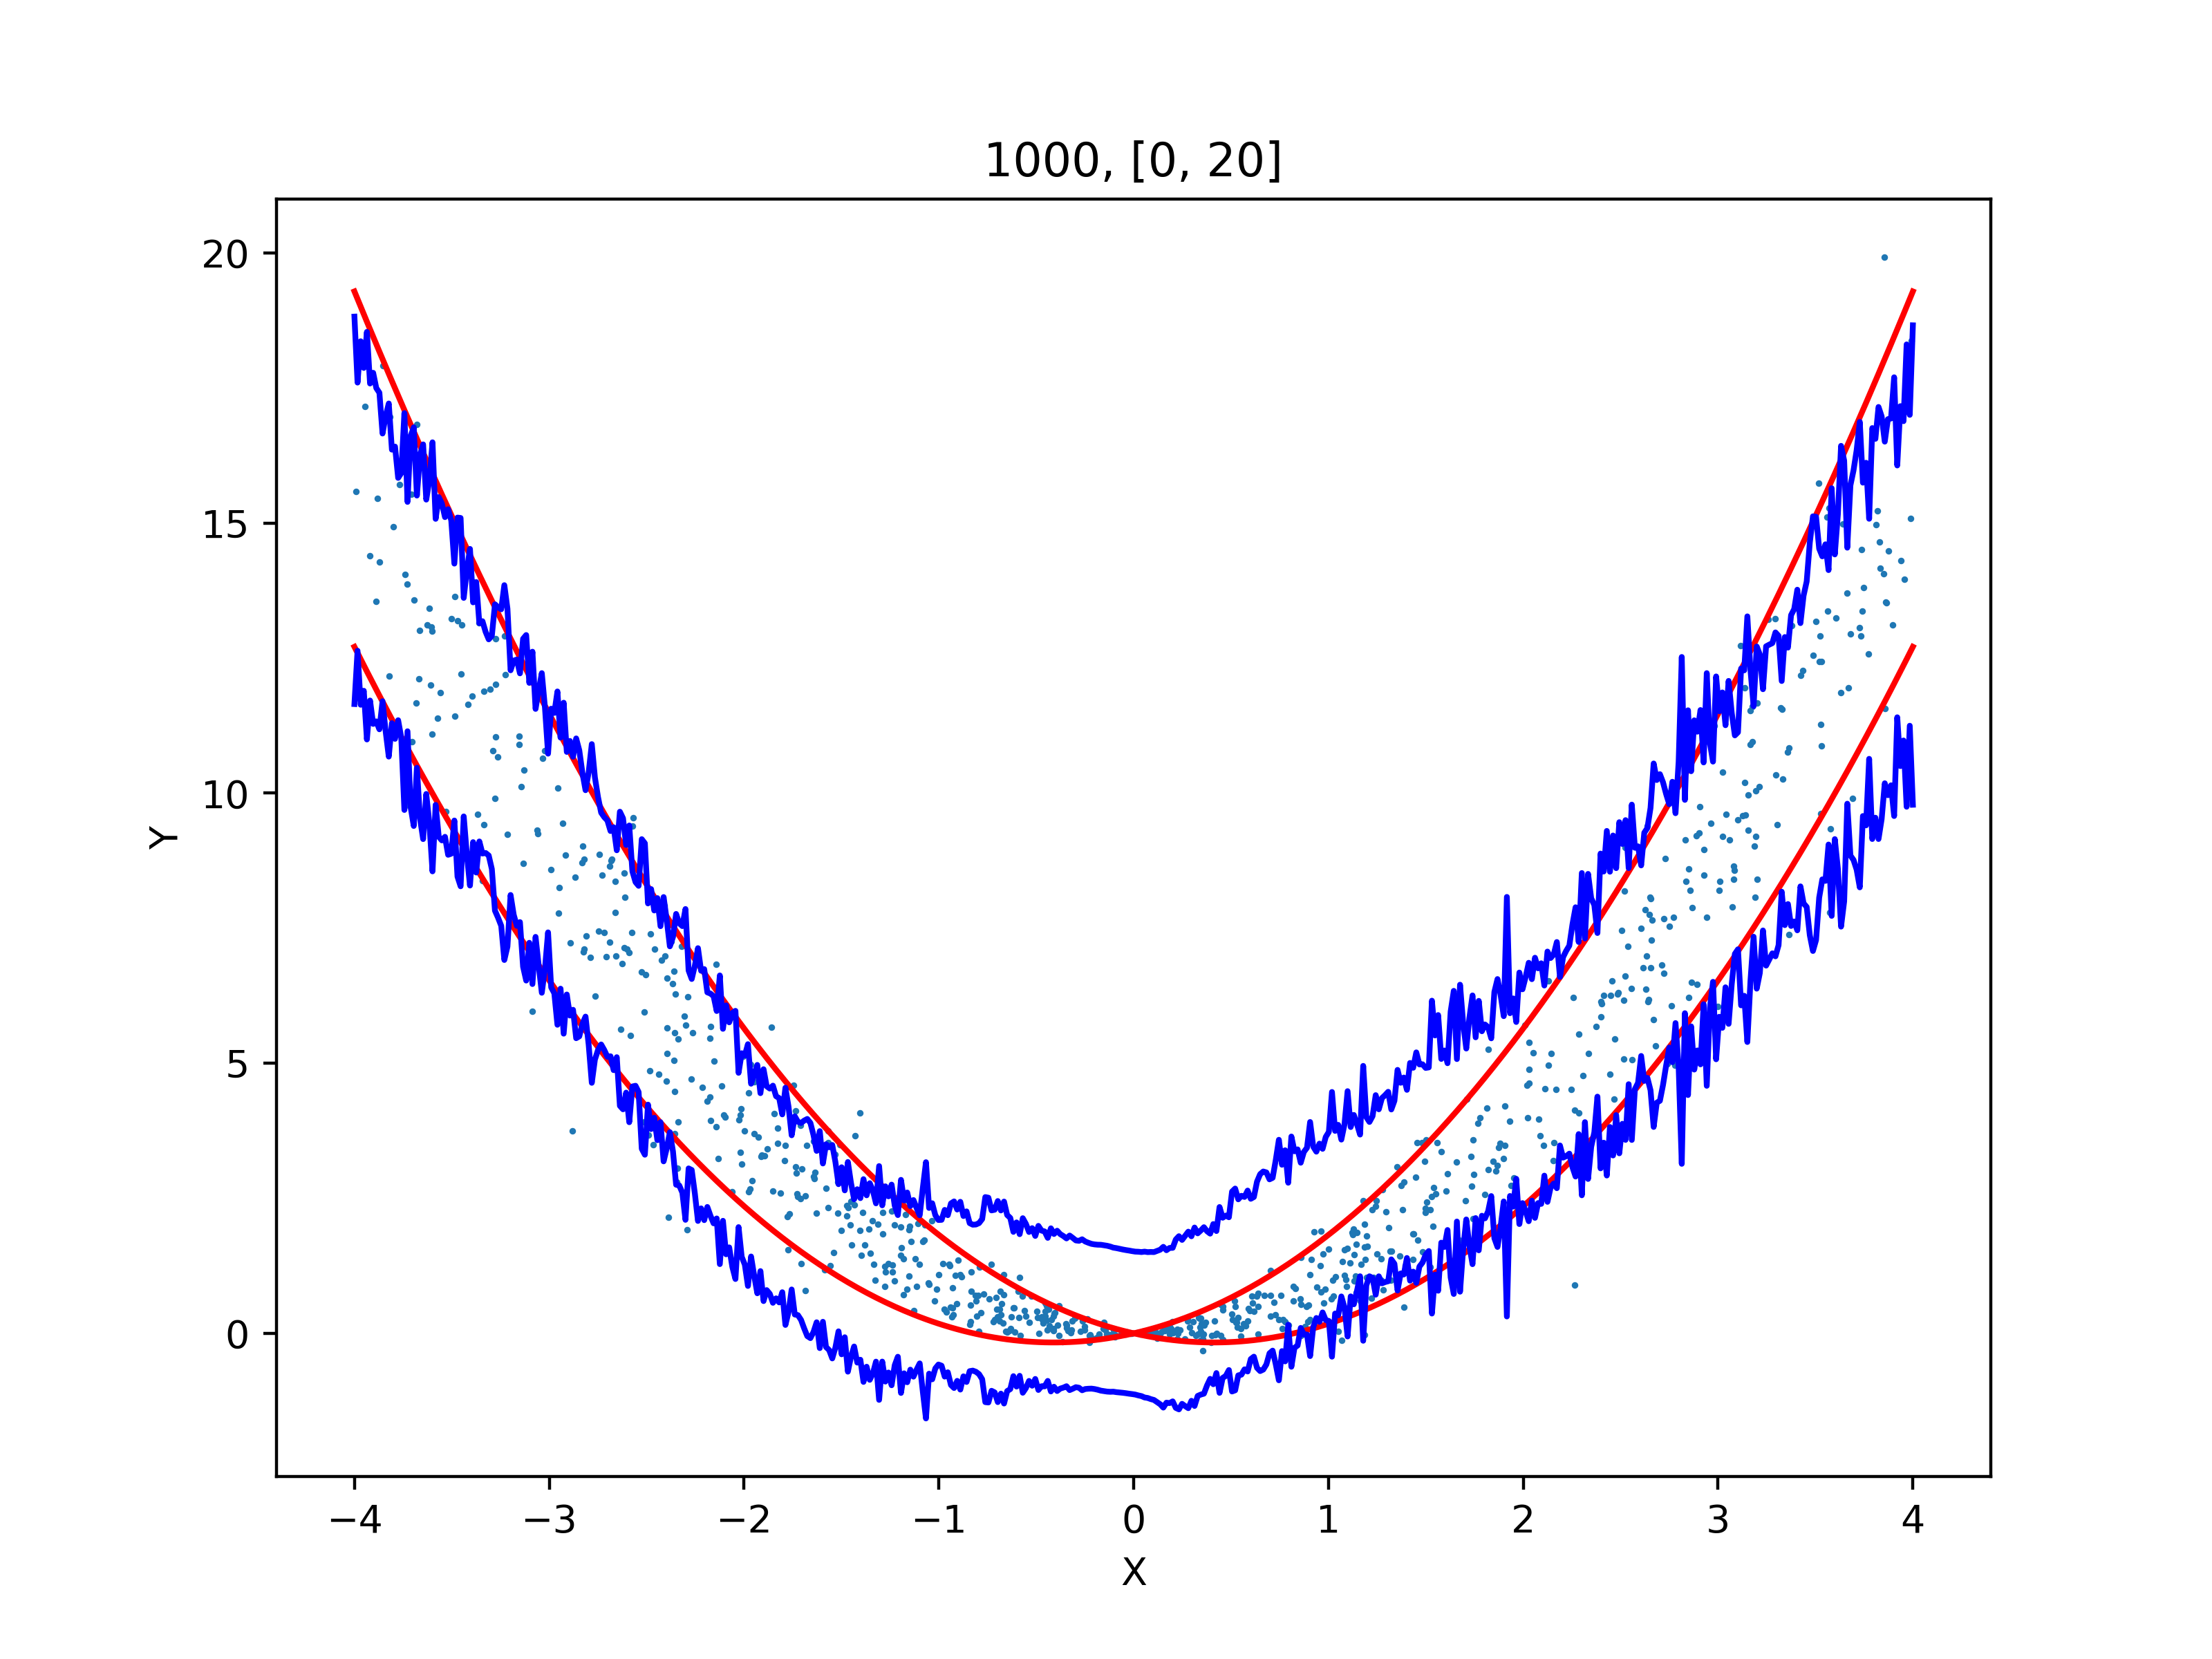
\includegraphics[width=0.98\linewidth]{fig/Ex1_1/0_20.png}
        \end{minipage}
        \caption{Fig2}
        \label{Fig2}
    \end{figure}

\subsection{Experiment2}
    Assume agent $k=1,\cdots,K$ each has $n$ samples $X_1^k,\cdots,X_n^k$ follow $N(\mu_k,9)$. Sythesize $Y_i^k=(X_i^k)^2+\epsilon$, where $\epsilon\sim N(0,(ep*|X|+ep*\theta_k)^2)$, $ep$ be some parameter and $\theta_k$ generated for each agent randomly between $1$ and $10$.
    \begin{itemize}
        \item $X$ has different distribution for each agents
        \item $EY|X$ is same for all agents
        \item $Y-EY|X$ has different distribution for different agents
    \end{itemize}

    The heterogeneity greatly influences the performance as this method treat data from different agents with same operation with respect to covariates. See in Fig \ref{Fig3}. $ep=h=0.5$.
    \begin{figure}[htbp]
        \centering
        \begin{minipage}{0.495\linewidth}
            \centering
            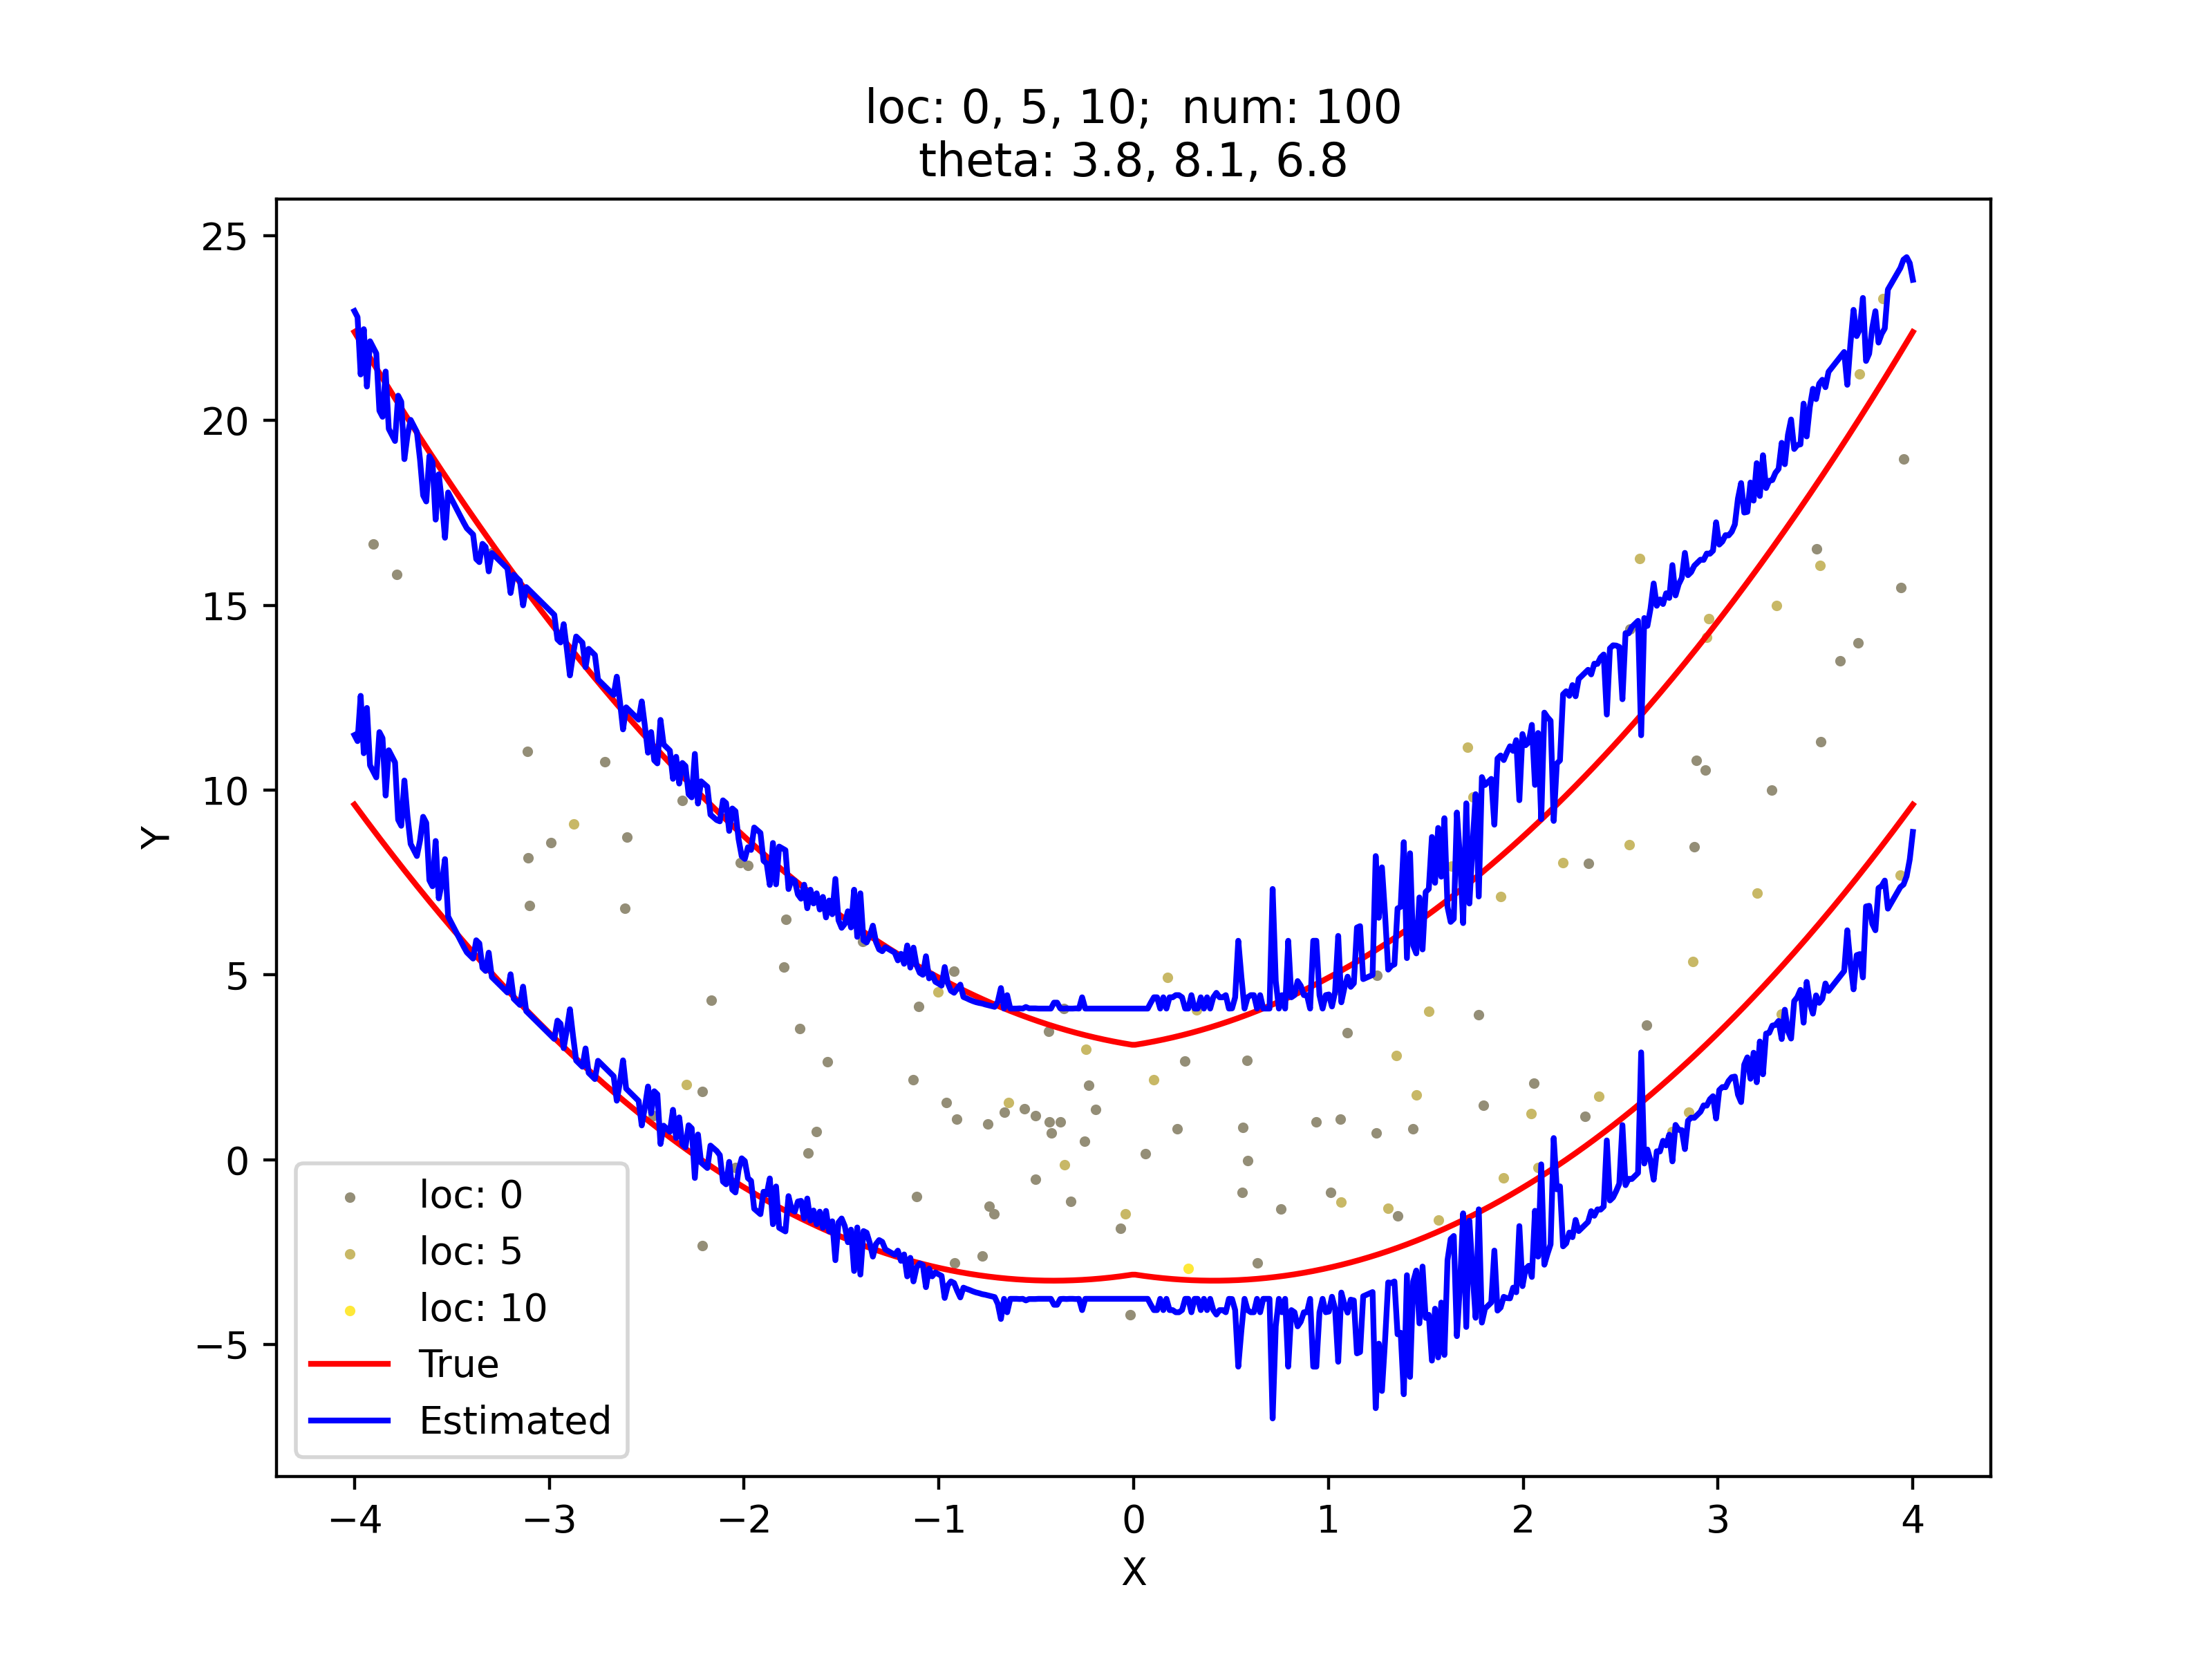
\includegraphics[width=0.98\linewidth]{fig/Ex1_2/0_5_10.png}
        \end{minipage}
        \begin{minipage}{0.495\linewidth}
            \centering
            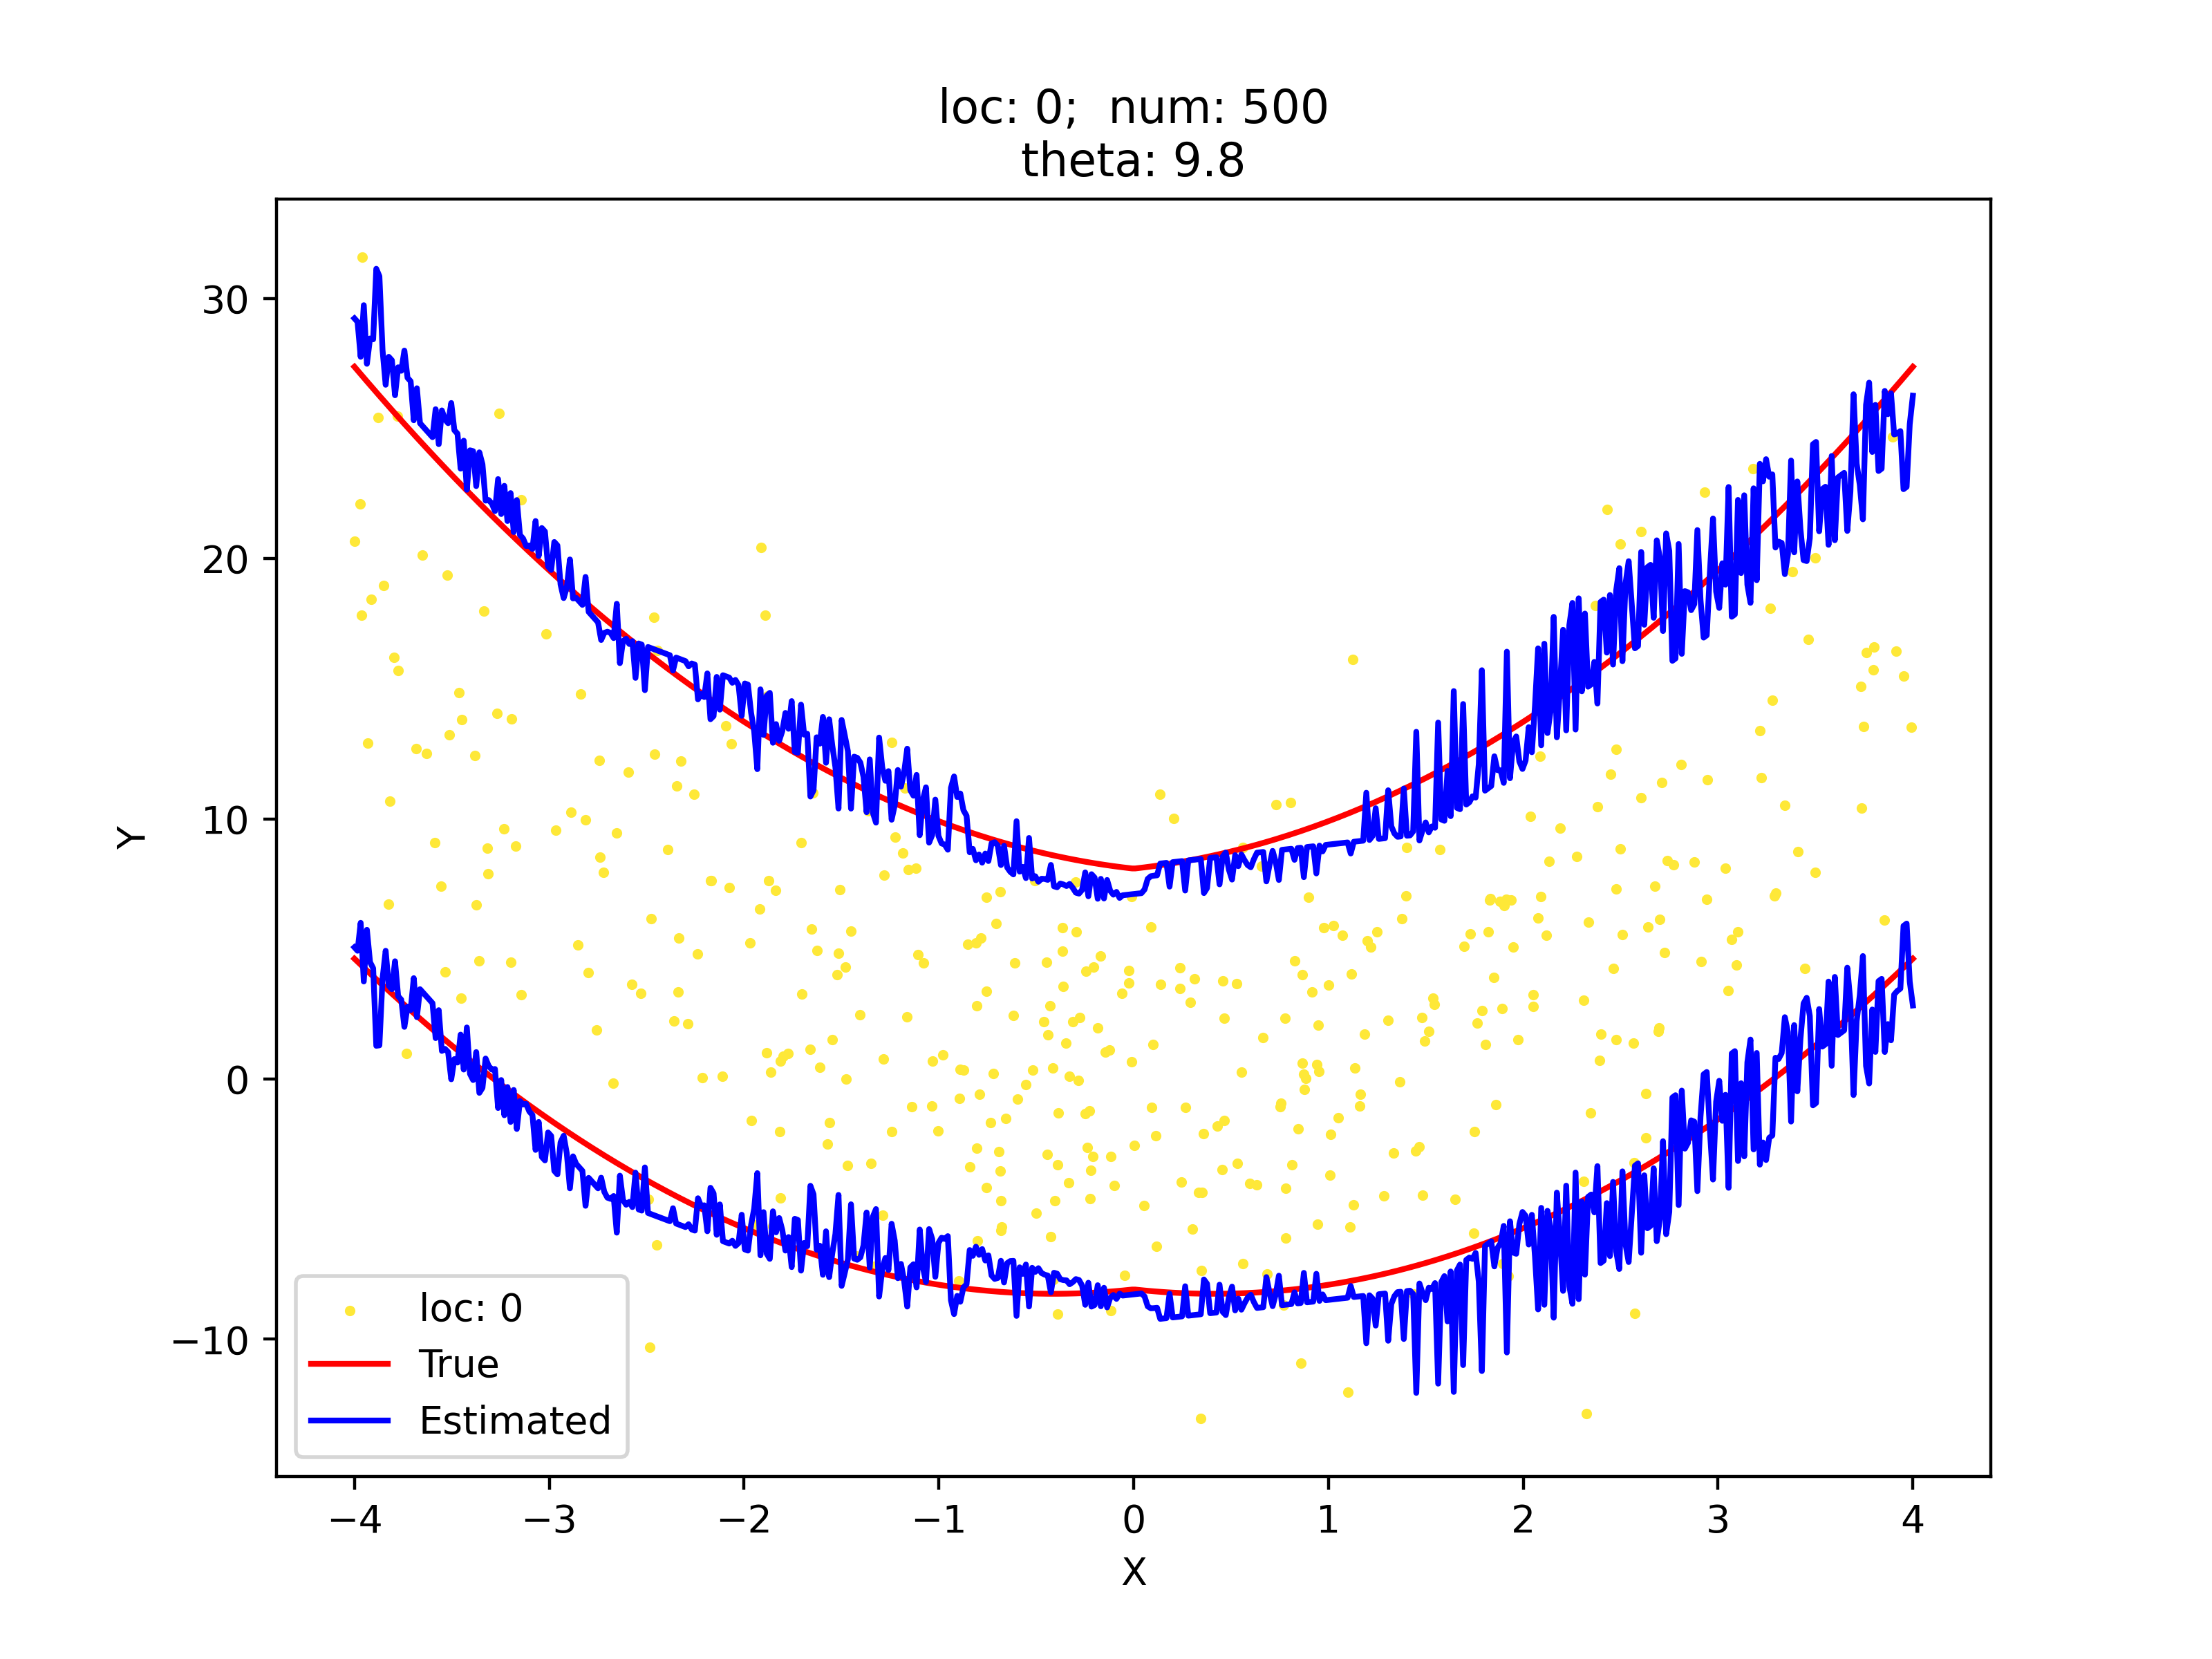
\includegraphics[width=0.98\linewidth]{fig/Ex1_2/0}
        \end{minipage}
        \centering
        \begin{minipage}{0.495\linewidth}
            \centering
            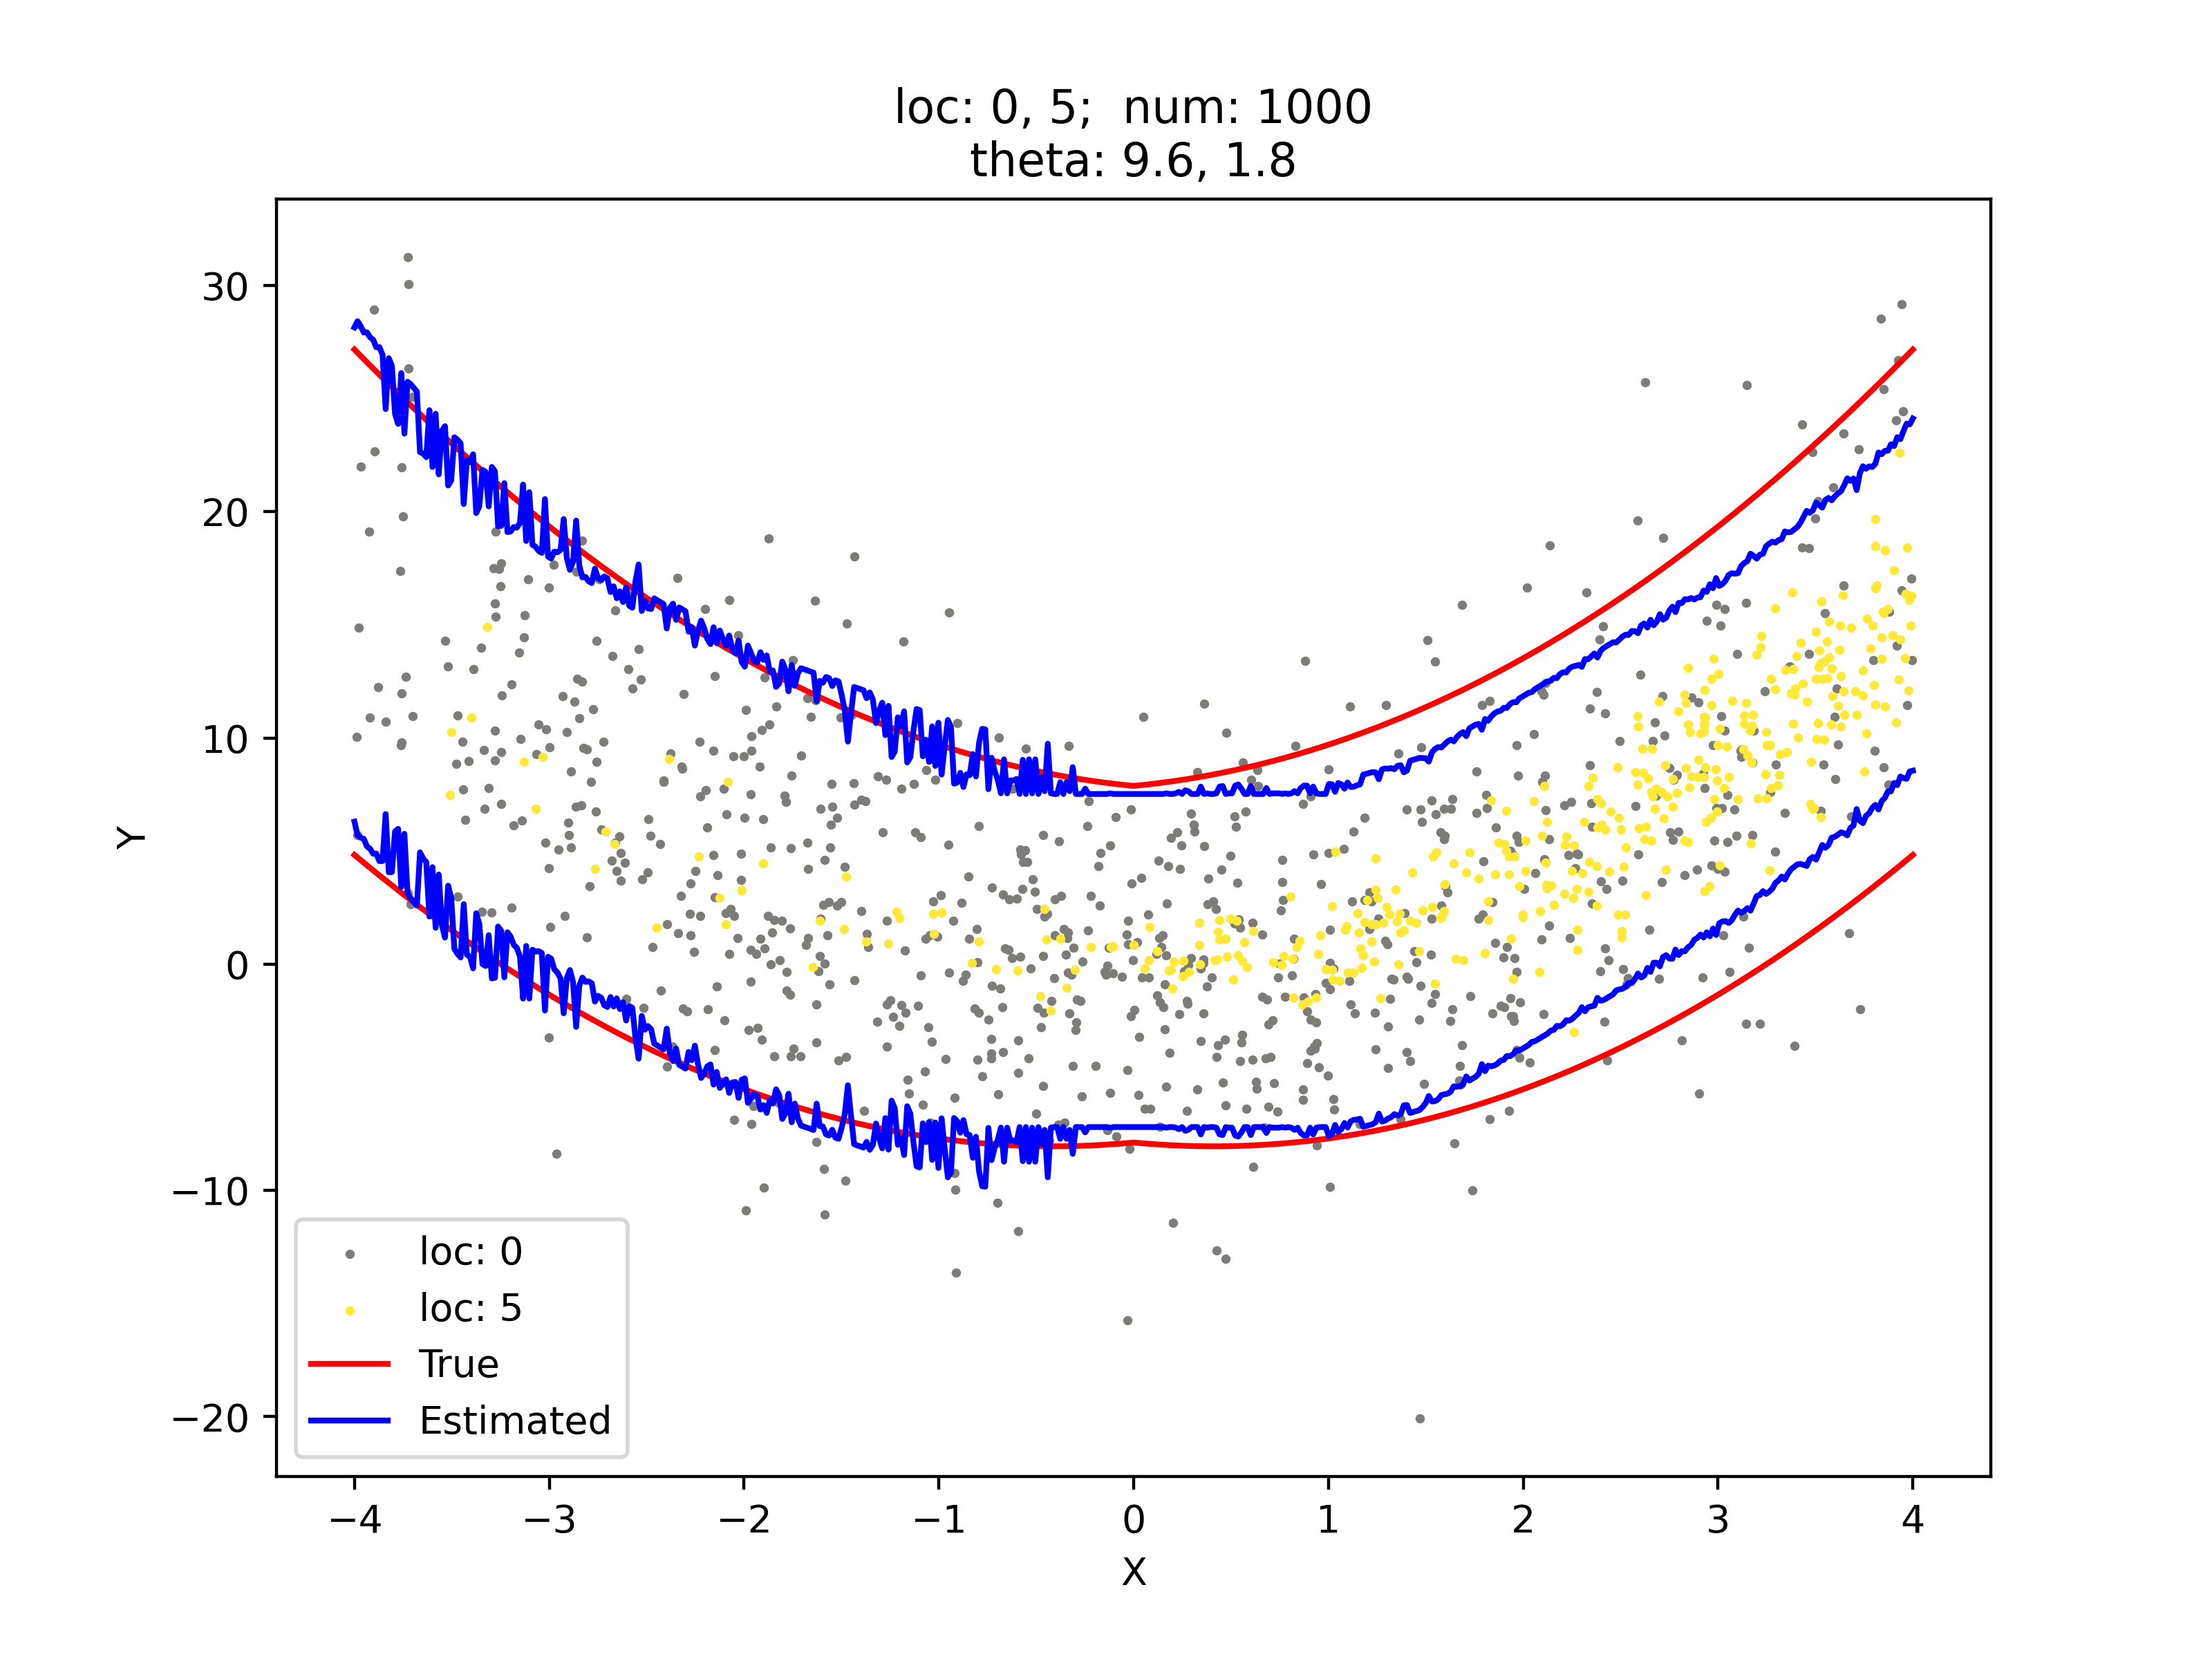
\includegraphics[width=0.98\linewidth]{fig/Ex1_2/0_5.png}
        \end{minipage}
        \begin{minipage}{0.495\linewidth}
            \centering
            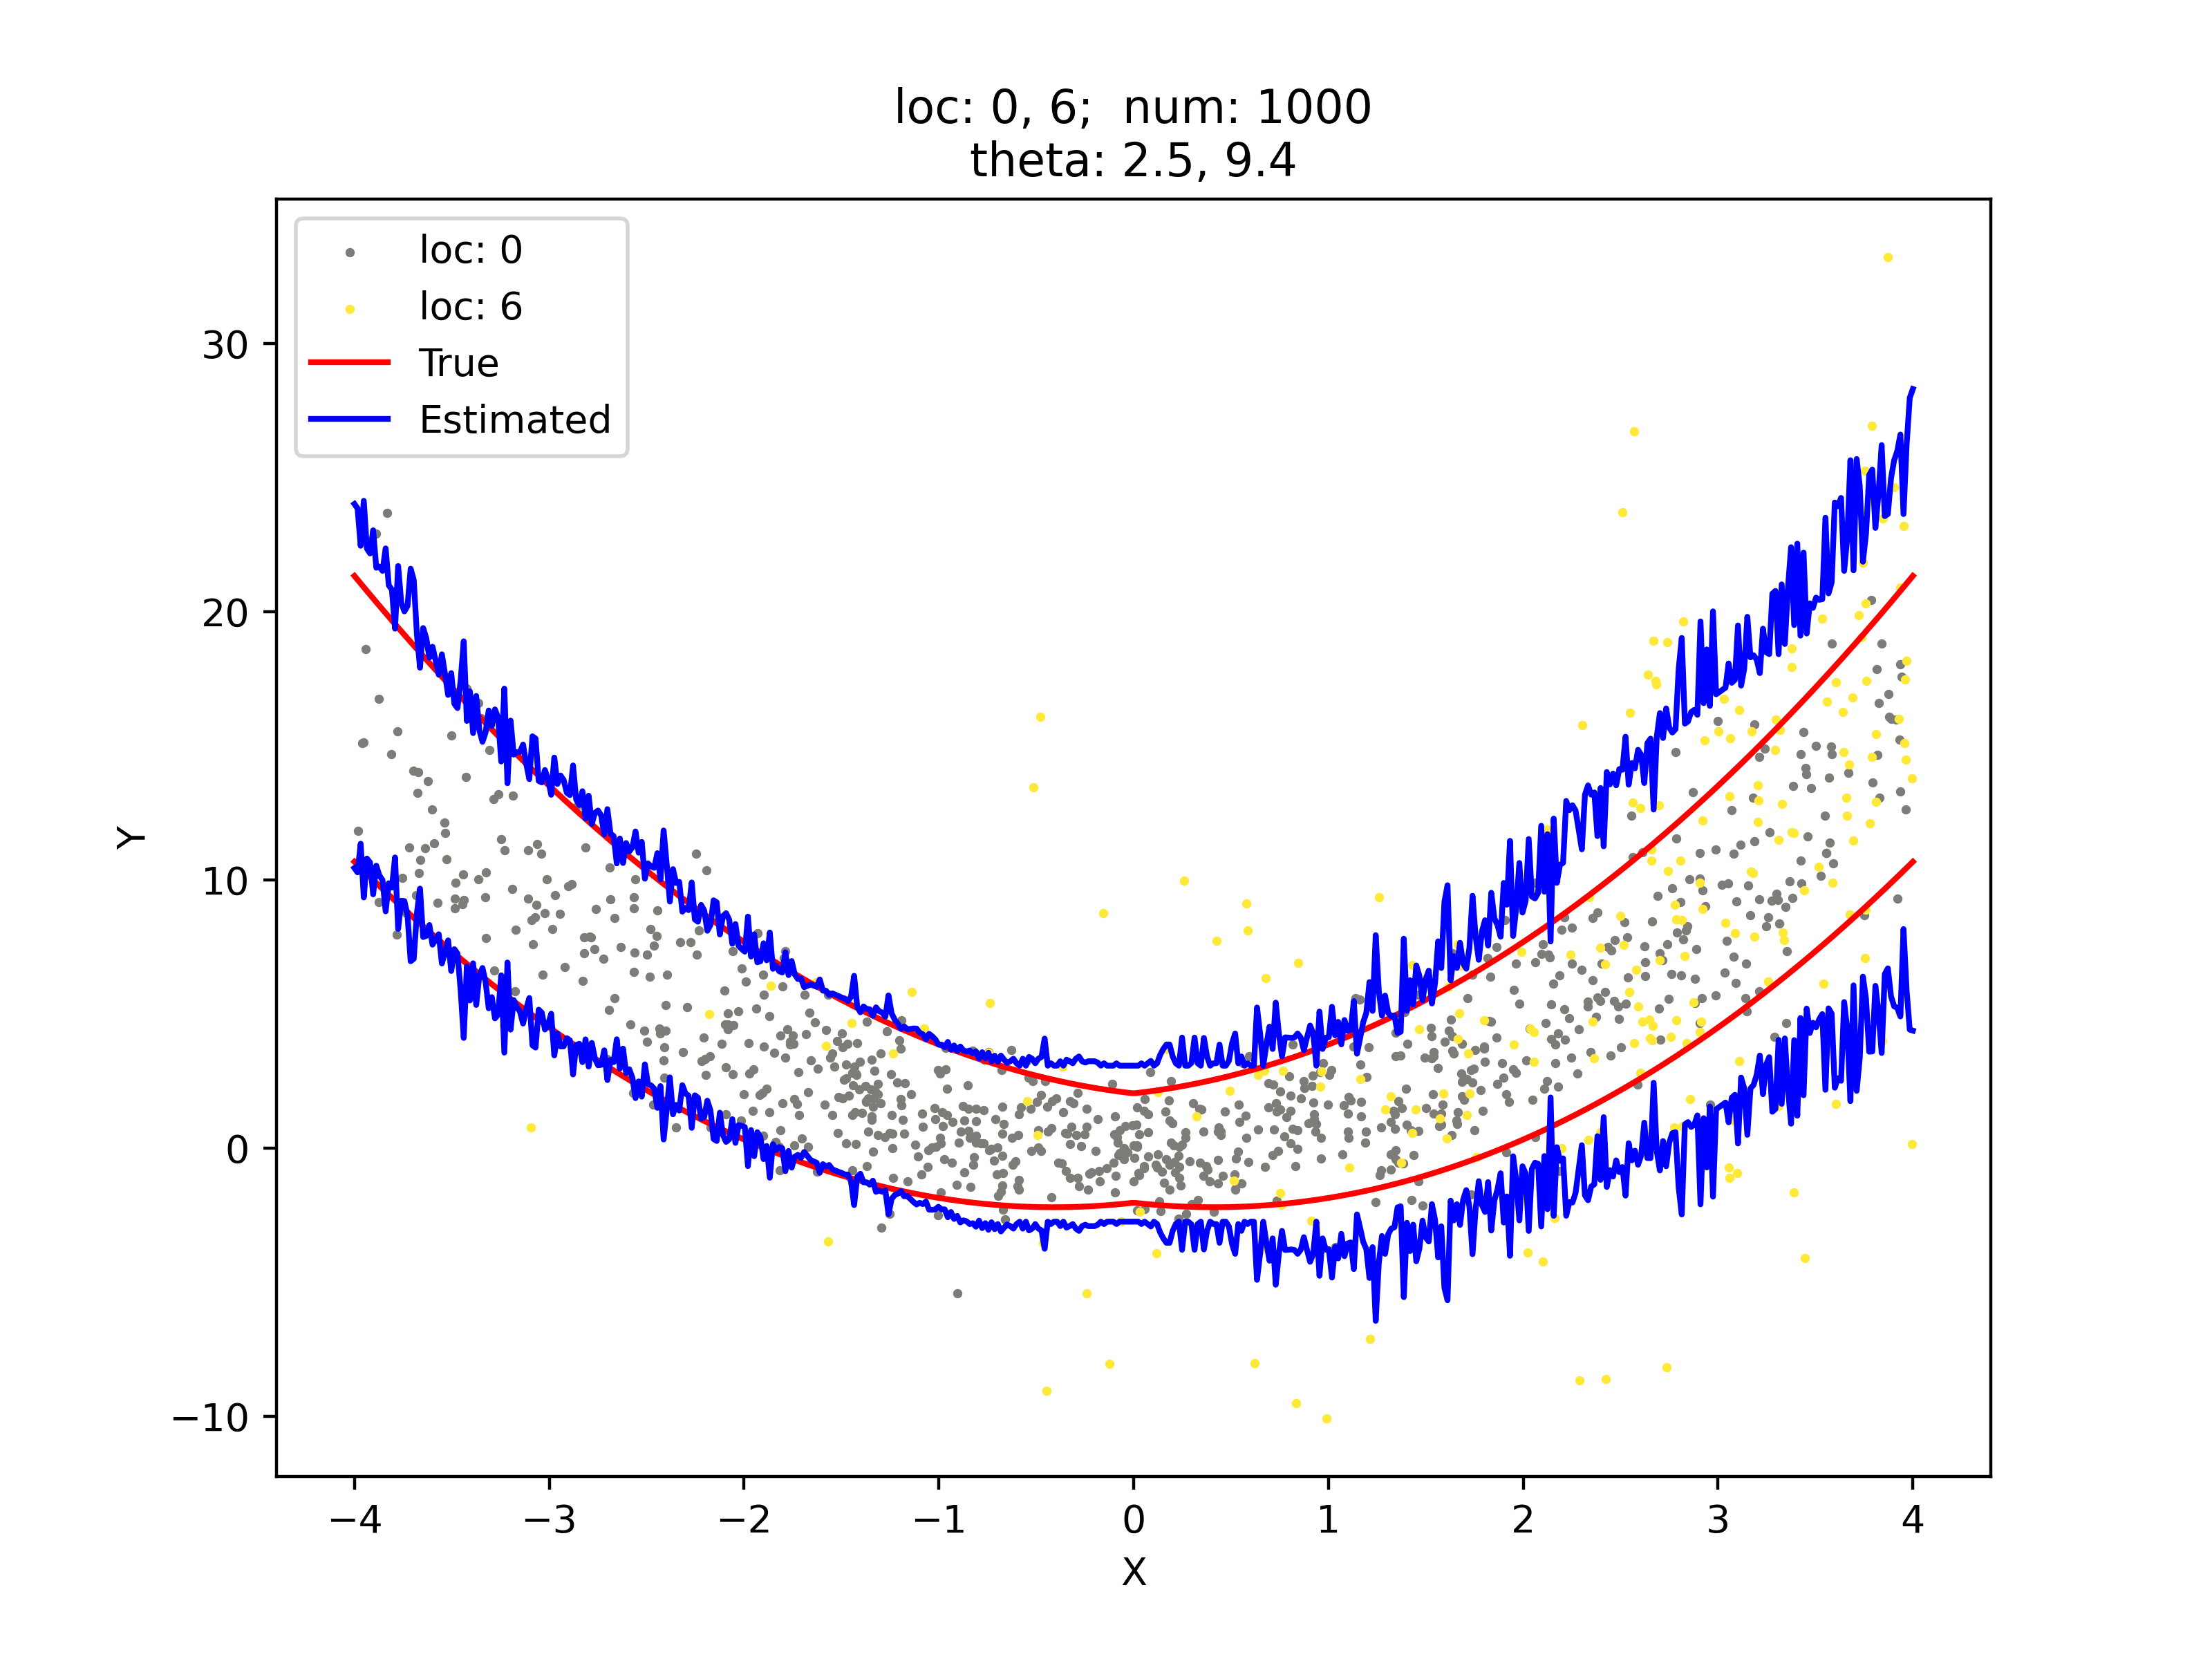
\includegraphics[width=0.98\linewidth]{fig/Ex1_2/0_6.png}
        \end{minipage}
        \caption{Fig3}
        \label{Fig3}
    \end{figure}


    To see how extra agent information influences performance, assume 4 agents with location 0, 5, 5, 10 and $\theta=(9.8, 2.1, 1.6, 6.3)$. Use only first agent data to estimate(left) and compare with the performance using all agents(right) in Fig \ref{Fig4}.
    \begin{figure}[htbp]
        \centering
        \begin{minipage}{0.495\linewidth}
            \centering
            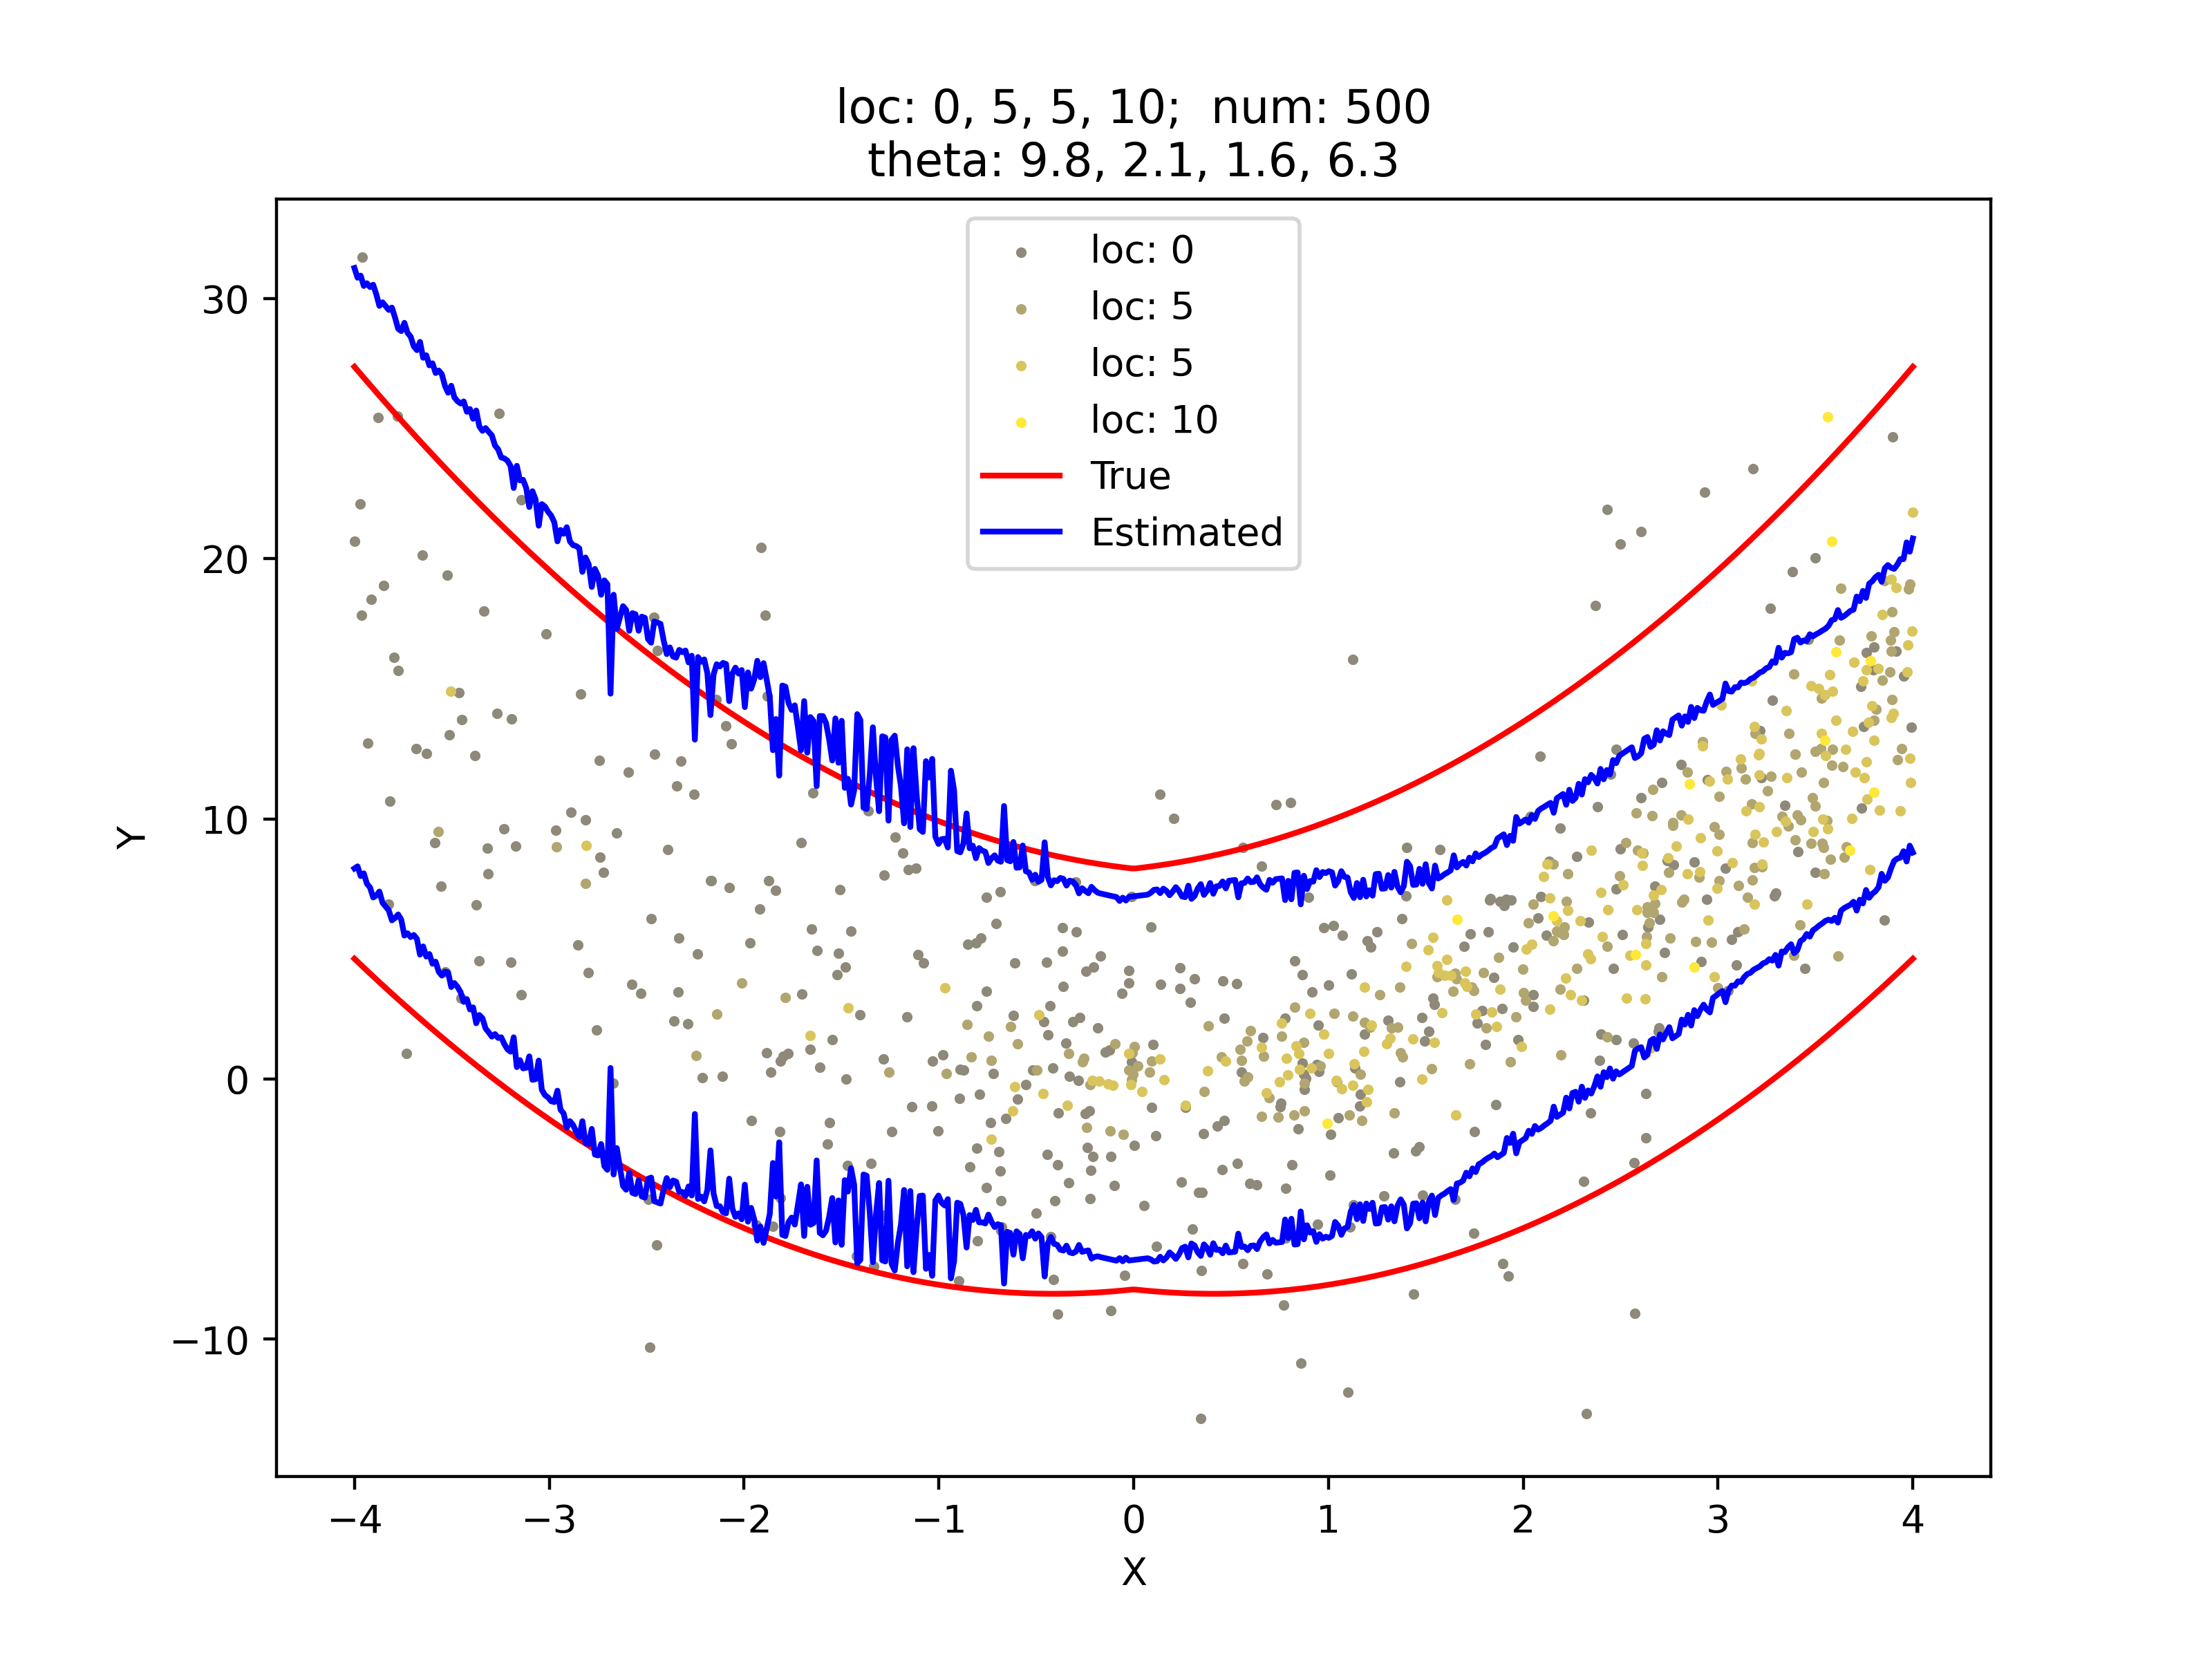
\includegraphics[width=0.98\linewidth]{fig/Ex1_2/0_5_5_10.png}
        \end{minipage}
        \begin{minipage}{0.495\linewidth}
            \centering
            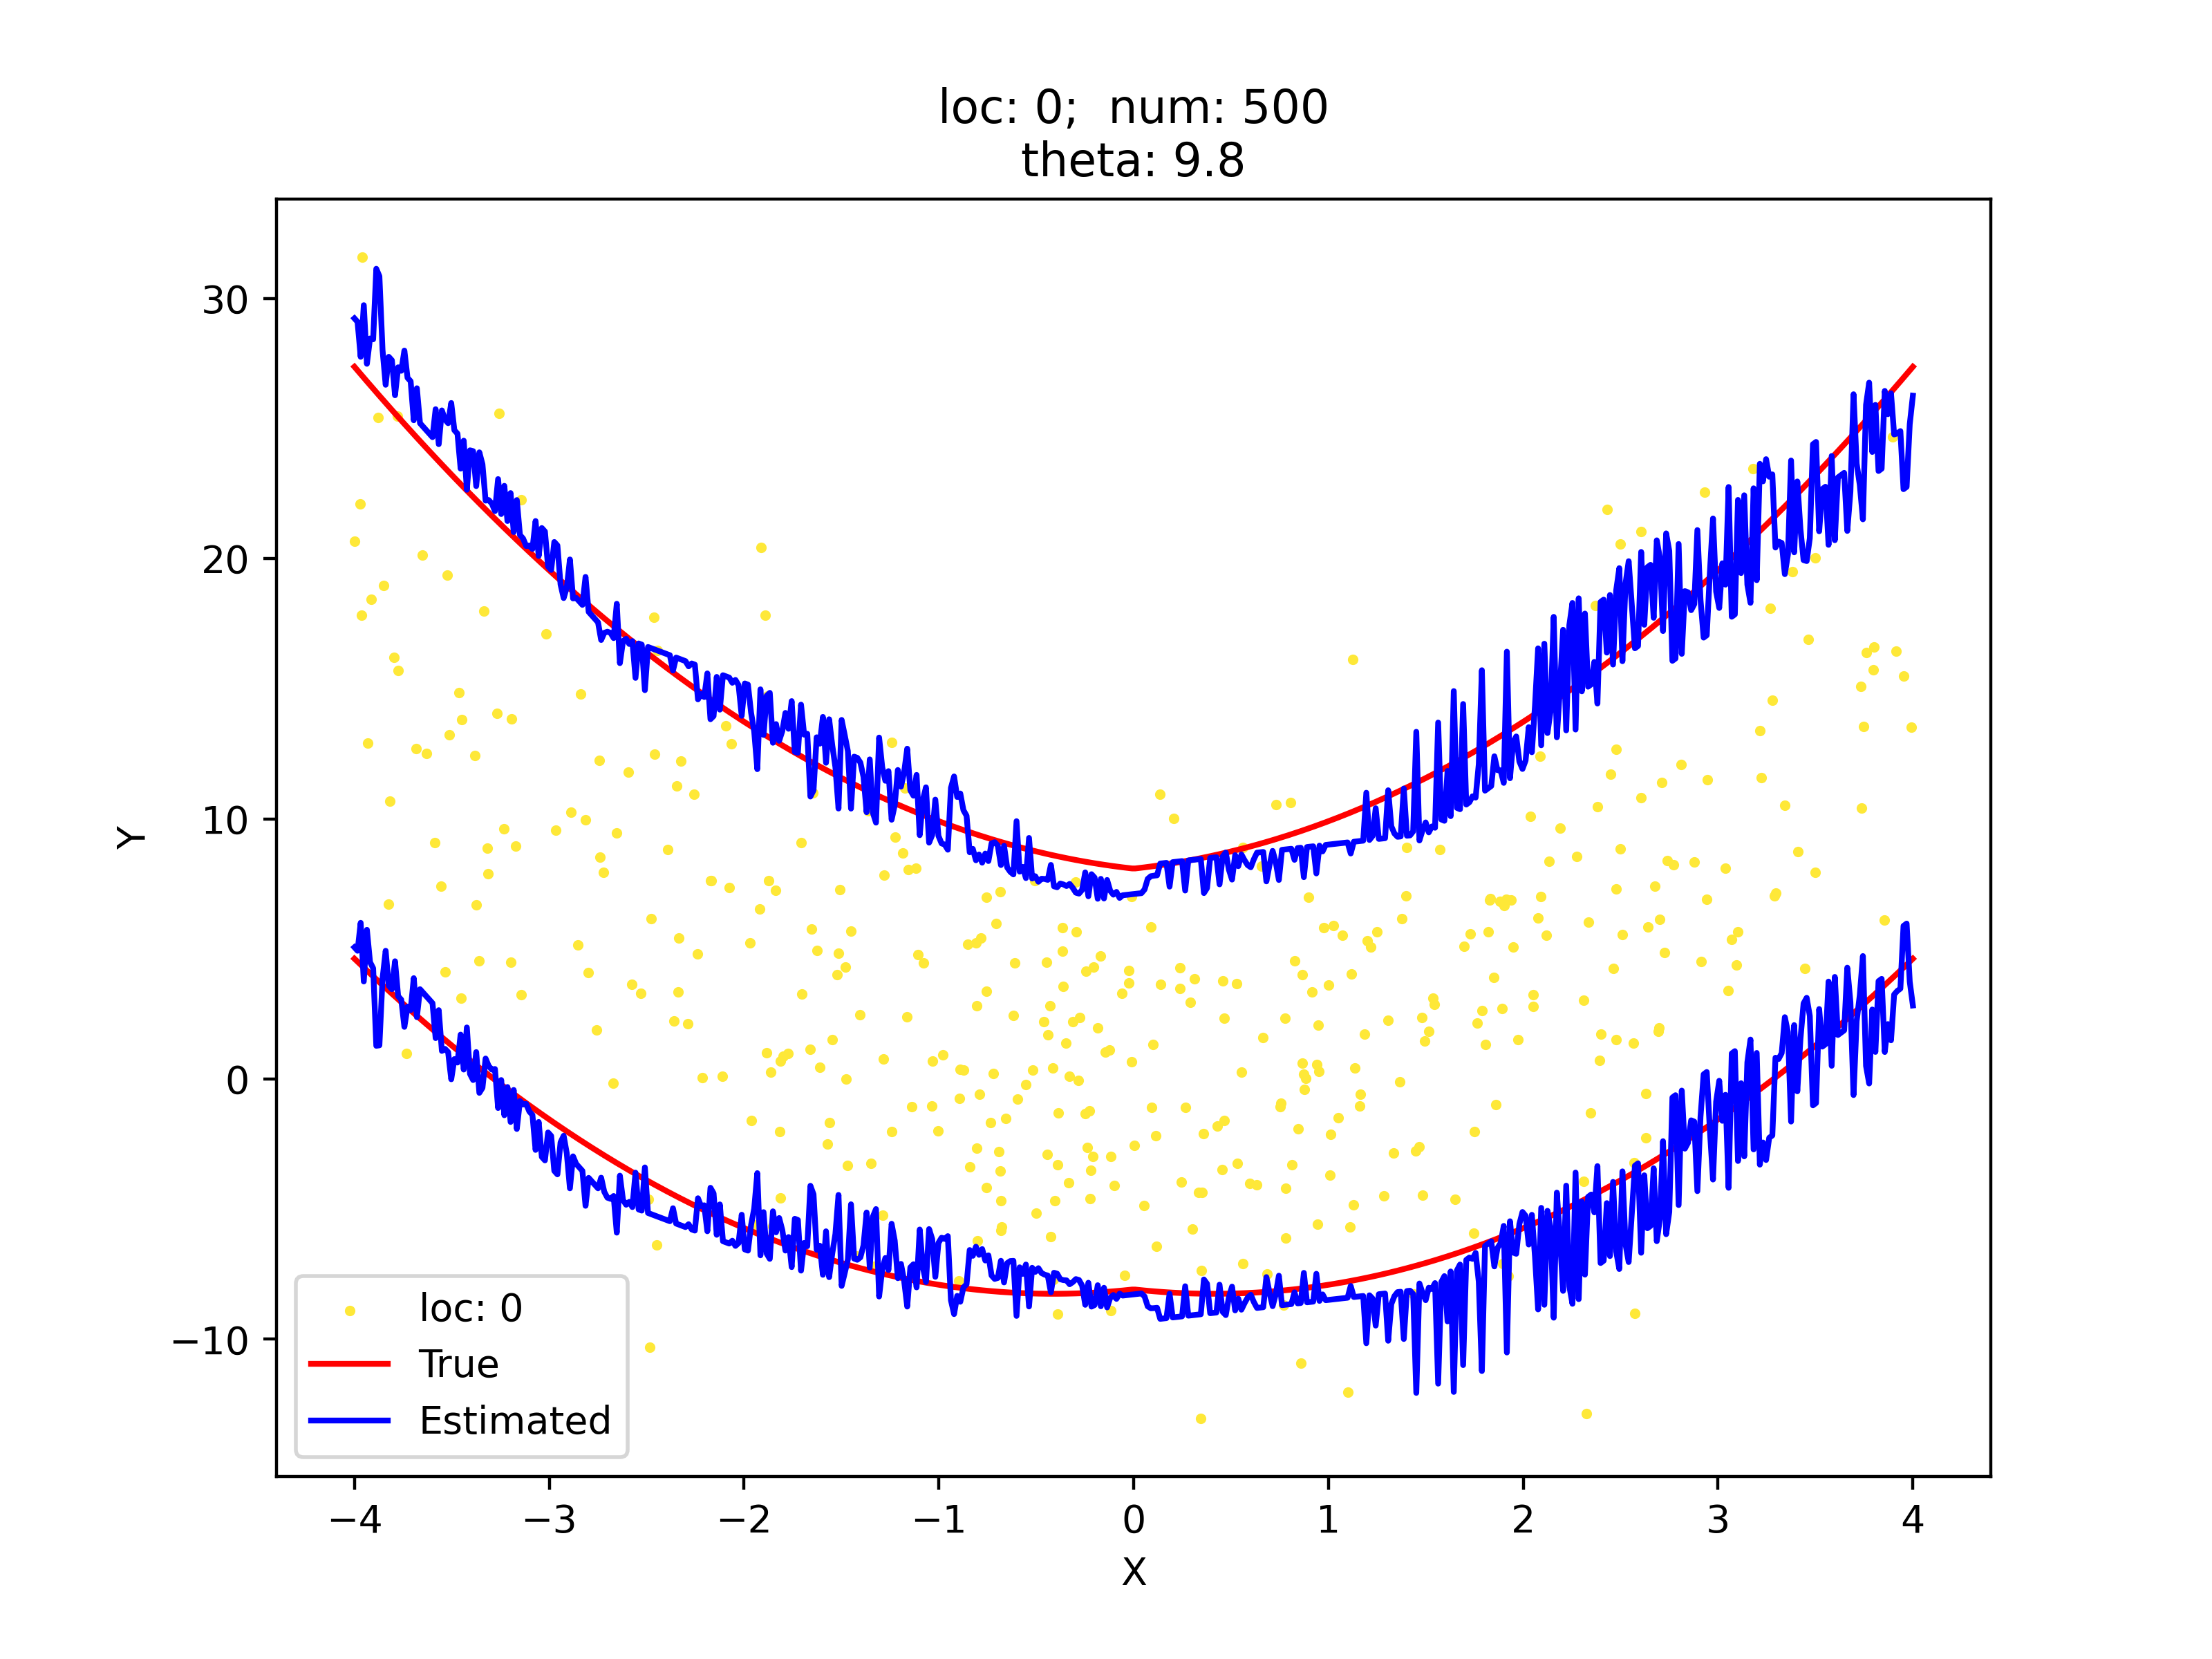
\includegraphics[width=0.98\linewidth]{fig/Ex1_2/0.png}
        \end{minipage}
        \caption{Fig4}
        \label{Fig4}
    \end{figure}


\newpage
\section{Idea2}
    This idea is based on Guan\cite{guan2023localized}.


    For $K$ agents each with $Z_k=\{Z_i^k=(X_i^k,Y_i^k)\}_{i=1}^{n_k}$ sampled from distribution $P^k$, and point predictor $f$ based score $S_i^k$.

    
    Given a new sample $X_{n_1+1}^1,Y_{n_1+1}^1$ from $P^1$, any trial data $y$ and $Z_{n_1+1}^1=(X_{n_1+1}^1,y)$. Now given some weight $p_{i,j}^{1,k}=\phi(Z_i^1,Z_j^k;Z_1,Z_k)$, where
    \begin{equation*}
        \phi(z,z';Z,Z'):\mathcal{Z}\times\mathcal{Z}\times\mathcal{Z}^{n}\times\mathcal{Z}^{n'}\rightarrow\mathbb{R},
    \end{equation*}
    is exchangeable within $Z$ and $Z'$ respectively. Construct
    \begin{equation*}
        \hat{F}_i^1=C_i\left[ \overset{K}{\underset{k=1}\sum}\overset{n_k}{\underset{j=1}\sum}p_{i,j}^{1,k}\delta_{S_j^k}+p_{i,n_1+1}^{1,1}\delta_{S_{n_1+1}^1} \right],\ i=1,\cdots,n_1+1.
    \end{equation*}


    Write $z_k=\{z_i^k=(x_i^k,y_i^k)\}_{i=1}^{n_k}$, corresponding score $s_i^k$, and $E_Z=\left\{ Z_1=z_1,\cdots,Z_K=z_K \right\}$. Write
    \begin{equation*}
        \hat{F}_i^{1'}=C_i\left[ \overset{K}{\underset{k=1}\sum}\overset{n_k}{\underset{j=1}\sum}p_{i,j}^{1,k}\delta_{s_j^k}+p_{i,n_1+1}^{1,1}\delta_{s_{n_1+1}^1} \right],\ i=1,\cdots,n_1+1.
    \end{equation*}
    Now calculate
    \begin{align*}
        &\mathbb{P}\left( S_{n_1+1}^1\leq Q(\alpha',\hat{F}_{n_1+1}^1)\Big|E_Z \right)\\
        \text{$Z_{n_1+1}^1$ is r.v}=&\overset{n_1+1}{\underset{i=1}\sum}\mathbb{P}\left( Z_{n_1+1}^1=z_i^1\Big|E_Z \right)\mathbbm{1}\left( S_{n_1+1}^1\leq Q(\alpha',\hat{F}_{n_1+1}^1)\Big|E_Z,S_{n_1+1}^1=z_i^1 \right)\\
        \text{Exchangeability of $Z_i^1$}=&\dfrac{1}{n_1+1}\overset{n_1+1}{\underset{i=1}\sum}\mathbbm{1}\left( S_{n_1+1}^1\leq Q(\alpha',\hat{F}_{n_1+1}^1)\Big|E_Z,Z_{n_1+1}^1=z_i^1 \right).
    \end{align*}
    Note the core idea lies here is that $\hat{F}_i^1$ is concentrated around point $X_i^1$. When $Z_{n_1+1}^1=Z_i^1$ and condition on $E_Z$, $\hat{F}_{n_1+1}^1=\hat{F}_i^{1'}$, thus
    \begin{align*}
        \mathbb{P}\left( S_{n_1+1}^1\leq Q(\alpha',\hat{F}_{n_1+1}^1)\Big|E_Z \right)=\dfrac{1}{n_1+1}\overset{n_1+1}{\underset{i=1}\sum}\mathbbm{1}\left( s_i^1\leq Q(\alpha',\hat{F}_i^{1'})\Big|E_Z \right).
    \end{align*}
    Find minimal $\alpha'$ makes $\dfrac{1}{n_1+1}\overset{n_1+1}{\underset{i=1}\sum}\mathbbm{1}\left( s_i^1\leq Q(\alpha',\hat{F}_i^{1'})\Big|E_Z \right)\geq 1-\alpha$, then we have
    \begin{equation*}
        \mathbb{P}\left( S_{n_1+1}^1\leq Q(\alpha',\hat{F}_{n_1+1}^1)\Big|E_Z \right)\geq 1-\alpha.
    \end{equation*}


\subsection{Method under Simplified Setting}
    However the previous process is very difficult to calculate, next is a practical implement. Simplify problem to $n$ samples $X_1,\cdots,X_n;Y_1,\cdots,Y_n$ and score $S_1,\cdots,S_n$ with new test point $X_{n+1}$. Assume scores are ordered such that $S_1\leq\cdots\leq S_n$ and $S_{l_i}$ is the biggest $S_j$ smaller than $S_i$. For example if $S_i>S_{i-1}$, $l_i=i-1$, define $l_1=0$. Given kernel function calculated weight $p_{i,j}$ based on $X_i,X_j$. $p_{i,j}=p_{j,i}$ and $\overset{n+1}{\underset{j=1}\sum}p_{i,j}=1$.
    \begin{itemize}
        \item Define $\theta_i$ be cumulative probability centered on $X_i$ till $l_i$, which is $\theta_i=\overset{l_i}{\underset{j=1}\sum}p_{i,j}$.
        \item Define $\tilde{\theta}_i$ be cumulative probability centered on $X_{n+1}$ till $l_i$, which is $\tilde{\theta}_i=\overset{l_i}{\underset{j=1}\sum}p_{n+1,j}$.
        \item Find three disjoint index sets
        \begin{align*}
            A_1&=\left\{ i:\tilde{\theta}_i>\theta_i+p_{n+1,i} \right\}\\
            A_2&=\left\{ i:\theta_i\geq\tilde{\theta}_i \right\}\\
            A_3&=\left\{ i:\theta_i<\tilde{\theta}_i\leq\theta_i+p_{n+1,i} \right\}
        \end{align*}
        \item Define following sets
        \begin{align*}
            B_1&=\left\{ \theta_i+p_{n+1,i}:i\in A_1 \right\}\\
            B_2&=\left\{ \theta_i:i\in A_2 \right\}\\
            B_3&=\left\{ l_i:i\in A_3 \right\}
        \end{align*}
        \item For $k=1,\cdots,n+1$ do following separately:
        \begin{itemize}
            \item Count $n_1,n_2$ be the number of items in $B_1,B_2$ that smaller than $\tilde{\theta}_k$, $n_3$ be the number of items in $B_3$ that smaller than $l(k)$.
            \item Define $T(k)=(n_1+n_2+n_3)/(n+1)$.
        \end{itemize}
        \item Find $k^*=\arg\max\left\{ k:S(k)<\alpha \right\}$. Take $S^*=S_{\min(n,k^*)}$.
        \item Construct conformal set $C_\alpha(X_{n+1})=\left\{ y:S_{n+1}\leq S^* \right\}$.
    \end{itemize}


\subsection{Method under Current Setting}
    Each agent $k=1,\cdots,K$ has $n_k$ labeled samples $Z_i^k=(X_i^k,Y_i^k)\sim P^k$, new test point $Z_{n_1+1}^1\sim P^1$ and all agents share common point estimator $f()$. Denote $S_i^k$ as the score. Construct
    \begin{gather*}
        \hat{F}_i^1(s)=\overset{K}{\underset{k=1}\sum}\overset{n_k}{\underset{j=1}\sum}p_{i,j}^{1,k}\delta_{S_j^k}+p_{i,n_1+1}^{1,1}\delta_s,\\
        C_S(X_{n_1+1})=\left\{ s:s\leq Q(\alpha(s);\hat{F}_{n_1+1}^1(\infty)) \right\},
    \end{gather*}
    where $\alpha(s)$ is the smallest number satisfies
    \begin{equation}
        \dfrac{1}{n_1+1}\overset{n_1+1}{\underset{j=1}\sum}\mathbbm{1}\left( S_j^1\leq Q(\alpha(s);\hat{F}_j^1(s)) \right)\geq \alpha.\label{alphas}
    \end{equation}


    \begin{lemma}
        Write $G=q_1\delta_{g_1}+\cdots+q_r\delta_{g_r}$, and assume $g_1\leq\cdots\leq g_r,q_1+\cdots+q_r=1$. We hava for any $\beta\in(0,1)$ and $t$
        \begin{equation*}
            \left\{ t\leq Q(\beta,G) \right\}\Leftrightarrow\left\{ \beta>\overset{}{\underset{i:g_i<t}\sum}q_i \right\}.
        \end{equation*}
    \end{lemma}


    \subsubsection{Method Deduction}
    By definition $s\in C_S(X_{n_1+1})\Leftrightarrow\alpha(s)>\overset{}{\underset{s_i^k<s}\sum}p_{n_1+1,i}^{1,k}\overset{def}{=}q(s)$. Assume $S_{i_2}^{k_2}<s<S_{i_1}^{k_1}$(take set closure ineq becomes eq). Denote
    \begin{gather*}
        \theta_j^1=\overset{}{\underset{S_i^k<S_j^1}\sum}p_{i,j}^{k,1}\\
        \tilde{\theta}_i^k=\overset{}{\underset{S_{i'}^{k'}<S_i^k}\sum}p_{n_1+1,i'}^{1,k'}=q(S_i^k).
    \end{gather*}
    Based on the smallest property of $\alpha(s)$ in formula (\ref{alphas}),
    \begin{equation*}
        s\in C_S(X_{n_1+1})\Leftrightarrow\dfrac{1}{n_1+1}\overset{n_1+1}{\underset{j=1}\sum}\mathbbm{1}\left( S_j^1\leq Q(q(s);\hat{F}_j^1(s)) \right)<\alpha
    \end{equation*}


    When $S_{i_2}^{k_2}<s<S_{i_1}^{k_1}$, it's easy to find $\overset{}{\underset{s_i^k<s}\sum}p_{n_1+1,i}^{1,k}=\tilde{\theta}_{i_1}^{k_1}$. First hope to prove
    \begin{equation}
        \left\{ S_j^1\leq Q(q(s);\hat{F}_j^1(s)) \right\}=\left\{ S_j^1\leq Q(\tilde{\theta}_{i_1}^{k_1};\hat{F}_j^1(s)) \right\}=\left\{ S_j^1\leq Q(\tilde{\theta}_{i_1}^{k_1};\hat{F}_j^1(\tilde{\theta}_{i_2}^{k_2})) \right\}.
    \end{equation}
    Only to prove the last equation.


    First notice that embedding $s$ into $\hat{F}_j^1$ makes
    \begin{gather}
        \left\{ S_j^1\leq Q(\tilde{\theta}_{i_1}^{k_1};\hat{F}_j^1(s)) \right\}=\left\{ \tilde{\theta}_{i_1}^{k_1}>\overset{}{\underset{S_i^k<S_j^1}\sum}p_{i,j}^{k,1} \right\}=\left\{
            \begin{aligned}
            &\left\{ \tilde{\theta}_{i_1}^{k_1}>\theta_j^1+p_{n_1+1,j}^{1,1} \right\},S_j^1\geq S_{i_1}^{k_1}\label{fiseq1}\\
            &\left\{ \tilde{\theta}_{i_1}^{k_1}>\theta_j^1 \right\},S_j^1<S_{i_1}^{k_1}.
            \end{aligned}
        \right.
    \end{gather}
    The $\overset{}{\underset{S_i^k<S_j^1}\sum}p_{i,j}^{k,1}$ is determined by the relationship between $s$ and $S_j^1$. When $s<S_j^1$ it equals to $\theta_j^1+p_{n_1+1,j}^{1,1}$, otherwise $\theta_j^1$.
    \begin{enumerate}
        \item $S_j^1\geq S_{i_1}^{k_1}$ leads to $S_j^1>s>S_{i_2}^{k_2}$ and this gives first formula in (\ref{fiseq1}). Finally
        \begin{equation*}
            \left\{ S_j^1\leq Q(\tilde{\theta}_{i_1}^{k_1};\hat{F}_j^1(\tilde{\theta}_{i_2}^{k_2})) \right\}=\left\{ \tilde{\theta}_{i_1}^{k_1}>\theta_j^1+p_{n_1+1,j}^{1,1} \right\}=\left\{ S_j^1\leq Q(\tilde{\theta}_{i_1}^{k_1};\hat{F}_j^1(s)) \right\}.
        \end{equation*}
        \item $S_j^1<S_{i_1}^{k_1}$, as $S_{i_2}^{k_2}$ is the next smallest beside $S_{i_1}^{k_1}$, leads to $S_j^1\leq S_{i_2}^{k_2}<s$. Thus gives second formula in (\ref{fiseq1}). Finally
        \begin{equation*}
            \left\{ S_j^1\leq Q(\tilde{\theta}_{i_1}^{k_1};\hat{F}_j^1(\tilde{\theta}_{i_2}^{k_2})) \right\}=\left\{ \tilde{\theta}_{i_1}^{k_1}>\theta_j^1 \right\}=\left\{ S_j^1\leq Q(\tilde{\theta}_{i_1}^{k_1};\hat{F}_j^1(s)) \right\}.
        \end{equation*}
    \end{enumerate}


    Now fix $i,k$ and the next smallest beside $S_{i}^{k}$ is $S_{i'}^{k'}$, $M_{j,i}^{1,k}=\left\{ S_j^1\leq Q(\tilde{\theta}_{i}^{k};\hat{F}_j^1(S_{i'}^{k'})) \right\}$. Split $M_{j,i}^{1,k}$ into two disjoint sets $M1_{j,i}^{1,k}$ and $M2_{j,i}^{1,k}$
    \begin{align*}
        M_{j,i}^{1,k}=&\left\{ S_{i'}^{k'}<S_j^1\leq Q(\tilde{\theta}_{i}^{k};\hat{F}_j^1(S_{i'}^{k'})) \right\}\cup\left\{ S_j^1\leq\min\left( S_{i'}^{k'},Q(\tilde{\theta}_{i}^{k};\hat{F}_j^1(S_{i'}^{k'})) \right) \right\}\\
        =&\left\{ S_{i'}^{k'}<S_j^1,\tilde{\theta}_{i}^{k}>\theta_j^1+p_{n_1+1,j}^{1,1} \right\}\cup\left\{ S_{i'}^{k'}\geq S_j^1,\tilde{\theta}_{i}^{k}>\theta_j^1 \right\}\\
        =&\left\{ S_{i}^{k}\leq S_j^1,\tilde{\theta}_{i}^{k}>\theta_j^1+p_{n_1+1,j}^{1,1} \right\}\cup\left\{ S_{i}^{k}>S_j^1,\tilde{\theta}_{i}^{k}>\theta_j^1 \right\}.
    \end{align*}


    Similar to simplified setting find three disjoint index sets
    \begin{align*}
        A_1&=\left\{ j:\tilde{\theta}_j^1>\theta_j^1+p_{n_1+1,j}^{1,1} \right\}\\
        A_2&=\left\{ j:\theta_i^1\geq\tilde{\theta}_j^1 \right\}\\
        A_3&=\left\{ j:\theta_j^1<\tilde{\theta}_j^1\leq\theta_j^1+p_{n_1+1,j}^{1,1} \right\}.
    \end{align*}
     

    \begin{enumerate}
        \item For $j\in A_1$, if $S_j^1<S_i^k$, directly we have $\tilde{\theta}_j^1<\tilde{\theta}_i^k$. As $j\in A_1$, $\tilde{\theta}_j^1>\theta_j^1+p_{n_1+1,j}^{1,1}$. Thus $\tilde{\theta}_{i}^{k}>\theta_j^1$ always hold. This means $\left\{ S_j^1<S_i^k,\tilde{\theta}_{i}^{k}\leq\theta_j^1+p_{n_1+1,j}^{1,1} \right\}=\emptyset$ and
        \begin{equation*}
            M_{j,i}^{1,k}=\left\{ S_j^1<S_i^k \right\}\cup\left\{ S_{i}^{k}\leq S_j^1,\tilde{\theta}_{i}^{k}>\theta_j^1+p_{n_1+1,j}^{1,1} \right\}=\left\{ \tilde{\theta}_{i}^{k}>\theta_j^1+p_{n_1+1,j}^{1,1} \right\}.
        \end{equation*}
        \item When $\tilde{\theta}_j^1\leq\theta_j^1+p_{n_1+1,j}^{1,1}$, if $S_i^k\leq S_j^1$, $\tilde{\theta}_i^k\leq\tilde{\theta}_j^1\leq\theta_j^1+p_{n_1+1,j}^{1,1}$ indicates $M1_{j,i}^{1,k}=\emptyset$ and $M_{j,i}^{1,k}=\left\{ S_{i}^{k}>S_j^1,\tilde{\theta}_{i}^{k}>\theta_j^1 \right\}$.
        \item For $j\in A_2$, $M_{j,i}^{1,k}=\left\{ S_{i}^{k}>S_j^1,\tilde{\theta}_{i}^{k}>\theta_j^1 \right\}$.
        \item For $j\in A_3$, when $S_i^k>S_j^1$, $\tilde{\theta}_{i}^{k}>\tilde{\theta}_{j}^{1}>\theta_j^1$ always hold. Thus $M_{j,i}^{1,k}=\left\{ S_{i}^{k}>S_j^1 \right\}$.
    \end{enumerate}
    In conclusion, given $k,i$, calculate $A_1,A_2,A_3$ and $S_{i'}^{k'}<s<S_{i}^{k}$,
    \begin{align}
        &\dfrac{1}{n_1+1}\overset{n_1+1}{\underset{j=1}\sum}\mathbbm{1}\left( S_j^1\leq Q(\tilde{\theta}_{i}^{k};\hat{F}_j^1(S_{i'}^{k'})) \right)\notag\\
        =&\dfrac{1}{n_1+1}\overset{}{\underset{j\in A_1\cup A_2\cup A_3}\sum}\mathbbm{1}\left( M_{j,i}^{1,k} \right)\notag\\
        =&\dfrac{1}{n_1+1}\left( \overset{}{\underset{j\in A_1}\sum}\mathbbm{1}\left( \tilde{\theta}_{i}^{k}>\theta_j^1+p_{n_1+1,j}^{1,1} \right)+\overset{}{\underset{j\in A_2}\sum}\mathbbm{1}\left( S_{i}^{k}>S_j^1,\tilde{\theta}_{i}^{k}>\theta_j^1 \right)+\overset{}{\underset{j\in A_3}\sum}\mathbbm{1}\left( S_{i}^{k}>S_j^1 \right) \right),\label{finalLen1}
    \end{align}
    indicates $s\in C_S(X_{n_1+1})\Leftrightarrow\text{(\ref{finalLen1})}<\alpha$. Find $S^*$ be the largest $S_i^k$ satisfies $\text{(\ref{finalLen1})}<\alpha$ and $C_S(X_{n_1+1})=[0,S^*]$.


    \subsubsection{Method Procedure}
    First all $Z_i^k,S_i^k,p_{j,i}^{1,k}$ are given.
    \begin{itemize}
        \item Calculate $\theta_j^1=\overset{}{\underset{S_i^k<S_j^1}\sum}p_{i,j}^{k,1},\tilde{\theta}_i^k=\overset{}{\underset{S_{i'}^{k'}<S_i^k}\sum}p_{n_1+1,i'}^{1,k'}=q(S_i^k)$
        \item Find index sets
        \begin{align*}
            A_1&=\left\{ j:\tilde{\theta}_j^1>\theta_j^1+p_{n_1+1,j}^{1,1} \right\}\\
            A_2&=\left\{ j:\theta_i^1\geq\tilde{\theta}_j^1 \right\}\\
            A_3&=\left\{ j:\theta_j^1<\tilde{\theta}_j^1\leq\theta_j^1+p_{n_1+1,j}^{1,1} \right\}.
        \end{align*}
        \item Order all $S_i^k$ and the $l$-th smallest denote as $S_{i(l)}^{k(l)}$. For $l=1,\cdots,N$ repeat
        \begin{align*}
            m_1&=\#\left\{ j\in A_1:\tilde{\theta}_{i(l)}^{k(l)}>\theta_j^1+p_{n_1+1,j}^{1,1} \right\}\\
            m_2&=\#\left\{ j\in A_2:S_{i(l)}^{k(l)}>S_j^1,\tilde{\theta}_{i(l)}^{k(l)}>\theta_j^1 \right\}\\
            m_3&=\#\left\{ j\in A_3:S_{i(l)}^{k(l)}>S_j^1 \right\}.
        \end{align*}
        Find $l^*$ be the largest $l$ makes $(m_1+m_2+m_3)/(n_1+1)<\alpha$.
        \item $C_S(X_{n+1})=[0,S_{i(l^*)}^{k(l^*)}]$
        \item Conformal set $C_\alpha(X_{n_1+1})=[f(X_{n_1+1})-S_{i(l^*)}^{k(l^*)},f(X_{n_1+1})+S_{i(l^*)}^{k(l^*)}]$.
    \end{itemize}
\newpage
\bibliographystyle{plain}
\bibliography{ref}
\end{document}